% !TEX TS-program = XeLaTeX
% use the following command:
% all document files must be coded in UTF-8
\documentclass[portuguese]{textolivre}
% build HTML with: make4ht -e build.lua -c textolivre.cfg -x -u article "fn-in,svg,pic-align"

\journalname{Texto Livre}
\thevolume{15}
%\thenumber{1} % old template
\theyear{2022}
\receiveddate{\DTMdisplaydate{2021}{11}{26}{-1}} % YYYY MM DD
\accepteddate{\DTMdisplaydate{2022}{1}{26}{-1}}
\publisheddate{\DTMdisplaydate{2022}{3}{2}{-1}}
\corrauthor{Mauricio Hinojosa}
\articledoi{10.35699/1983-3652.2022.37275}
%\articleid{NNNN} % if the article ID is not the last 5 numbers of its DOI, provide it using \articleid{} commmand
\runningauthor{Hinojosa et al.} 
%\editorname{Leonardo Araújo} % old template
\sectioneditorname{Hugo Heredia Ponce}
\layouteditorname{Leonado Araújo}

\title{Procedimiento de agrupación de estudiantes según riesgo de abandono para mejorar la gestión estudiantil en educación superior}
\othertitle{Procedimento de agrupamento de alunos de acordo com o risco de evasão para melhorar a gestão estudantil no ensino superior}
\othertitle{Student clustering procedure according to dropout risk to improve student management in higher education}

\author[1]{Mauricio~Hinojosa~\orcid{0000-0002-8962-7517}~\thanks{Email:~mauricio.hinojosa@usach.cl}}
\author[1]{Iván~Derpich~\orcid{0000-0001-9759-7285}~\thanks{Email:~ivan.derpich@usach.cl}} 
\author[1]{Miguel~Alfaro~\orcid{0000-0001-5891-8859}~\thanks{Email:~miguel.alfaro@usach.cl}}
\author[2]{David~Ruete~\orcid{0000-0002-7100-9737}~\thanks{Email:~druete@unab.cl}}
\author[2]{Alejandro~Caroca~\orcid{0000-0002-1191-687X}~\thanks{Email:~acaroca@unab.cl}}
\author[2]{Gustavo~Gatica~\orcid{0000-0002-1816-6856}~\thanks{Email:~ggatica@unab.cl}}
\affil[1]{Universidad de Santiago de Chile, Facultad de Ingeniería, Departamento de Ingeniería Industrial, Santiago, Región Metropolitana, Chile.}
\affil[2]{Universidad Andrés Bello, Facultad de Ingeniería, Santiago, Región Metropolitana, Chile.}


\addbibresource{article.bib}

% if you use multirows in a table, include the multirow package
\usepackage{multirow}

\begin{document}
\maketitle

\begin{polyabstract}
\begin{abstract}
La compleja problemática del abandono estudiantil representa una oportunidad para la aplicación de la tecnología y métodos de la minería de datos en educación superior. El objetivo de esta investigación es obtener el perfil de los estudiantes en riesgo de abandono y así generar planes de gestión estudiantil que impacten sobre las variables que explican esta situación. Para esto se propone utilizar una estructura metodológica CRISP-DM, aplicando herramientas estadísticas y del aprendizaje automático no supervisado. El análisis, de tipo transversal, se realizó sobre un universo de estudiantes de primer año en jornada diurna, en una universidad privada chilena. Las variables sociodemográficas y de comportamiento utilizadas, se basaron en la teoría sobre deserción y juicio de expertos, y los datos se obtuvieron de los registros históricos disponibles en la Institución. Para obtener las variables que más influían en el abandono se realizaron análisis de correlación y de componentes principales. La aplicación del clustering jerárquico aglomerativo y la técnica de conjuntos aproximados produjeron cuatro perfiles de estudiantes con sus reglas de asociación respectivas y cinco variables académicas que permitieron diseñar un sistema de apoyo para disminuir el abandono y fomentar la retención.

\keywords{Abandono estudiantil \sep CRISP-DM \sep Análisis de componentes principales \sep Clustering jerárquico aglomerativo \sep Conjuntos aproximados}
\end{abstract}

% Segundo resumen. En portugués.
\begin{portuguese}
\begin{abstract}
O complexo problema da evasão de alunos representa uma oportunidade para a aplicação de tecnologia e métodos de mineração de dados no ensino superior. O objetivo desta pesquisa é obter o perfil dos alunos em risco de evasão e, assim, gerar planos de gestão estudantil que impactem nas variáveis que explicam essa situação. Para isso, propõe-se a utilização de uma estrutura metodológica CRISP-DM, aplicando ferramentas estatísticas e aprendizado de máquina não supervisionado. A análise transversal foi realizada em um universo de alunos do primeiro ano do turno diurno de uma universidade privada chilena. As variáveis sociodemográficas e comportamentais utilizadas foram baseadas na teoria da deserção e no julgamento de especialistas, e os dados foram obtidos nos registros históricos disponíveis na Instituição. Para obter as variáveis que mais influenciaram o abandono, foram realizadas análises de correlação e de componentes principais. A aplicação do agrupamento hierárquico aglomerativo e da técnica de conjuntos aproximados produziu quatro perfis de alunos com suas respectivas regras de associação e cinco variáveis acadêmicas que permitiram desenhar um sistema de apoio para reduzir o abandono e promover a retenção.

\keywords{Evasão escolar \sep CRISP-DM \sep Análise de componentes principais
\sep Agrupamento hierárquico aglomerativo \sep Conjuntos aproximados}
\end{abstract}
\end{portuguese}

% Tercer resumen. En inglés.
\begin{english}
\begin{abstract}
The complex problem of student dropout represents an opportunity for the application of data mining technology and methods in higher education. The objective of this research is to obtain the profile of students at risk of dropping out and thus generate student management plans that impact on the variables that explain this situation. For this, it is proposed to use a CRISP-DM methodological structure, applying statistical tools and unsupervised machine learning. The cross-sectional analysis was carried out on a universe of freshmen day students at a private Chilean university. The sociodemographic and behavioural variables used were based on attrition theory and expert judgment, and the data were obtained from the historical records available at the Institution. To obtain the variables that most influenced dropout, correlation and principal component analyses were performed. The application of agglomerative hierarchical clustering and rough sets technique produced four profiles of students with their respective association rules and five academic variables that allowed the design of a support system to reduce dropout and promote retention.

\keywords{Student dropout \sep CRISP-DM \sep Principal component analysis
\sep Agglomerative hierarchical clustering \sep Rough sets}
\end{abstract}
\end{english}

\end{polyabstract}

% CUERPO DEL ARTÍCULO;

\section{Introducción}\label{sec-intro}

La deserción o abandono estudiantil es un problema reconocido y estudiado mundialmente en la educación \cite{ProyectoAlfaGuia}, impacta en la efectividad, eficiencia y prestigio de los sistemas e instituciones educacionales, y puede generar consecuencias económicas y/o psicosociales negativas en los estudiantes y sus familias \cite{Schreiber2020,OECD2009b}.

Con la tendencia hacia la universalización de la Educación Superior (ES), una mayor proporción del alumnado proviene de los sectores socioeconómicos más vulnerables, cuya preparación académica muchas veces es deficiente, y deben compatibilizar estudios y trabajo \cite{HinojosaV2021}. Esto genera un mayor abandono en este grupo socioeconómico, que se refleja en una menor tasa de finalización que perjudica el acceso con equidad \cite{Ferreyra2017,ServiciodeInformaciondeEducacionSuperiorSIES2014}. Además, la pandemia del COVID-19 aumenta la probabilidad de abandonar de estos estudiantes debido a una inevitable reducción en la calidad del proceso de enseñanza/aprendizaje \cite{OECD2021}.

En Latinoamérica, los sistemas de acreditación y/o aseguramiento de la calidad ya consideran este fenómeno \cite{LemaitreIESALC2017}. En el caso de Chile, su Sistema Nacional de Aseguramiento de la Calidad \cite{Ministeriodeeducacion2006} incluye un proceso de acreditación, el cual, según la nueva Ley de Educación Superior, exige a las instituciones de educación superior (IES) acreditarse, entre otros, en el ámbito de la docencia y resultados del proceso formativo \cite{Ministeriodeeducacion2018}. En base a lo anterior, la Comisión Nacional de Acreditación (CNA) propone criterios y estándares de evaluación, donde destacan que IES posean procedimientos definidos de seguimiento y análisis de retención. Para pregrado (CINE 5 y 6) \cite{UNESCOInstituteforStatistics2012} definen como estándar mínimo una tasa de retención institucional de primer año mayor o igual a 65~\%, o que la institución presente una tasa de retención de cohorte al término del tercer año, mayor o igual a 60~\% \cite{ServiciodeInformaciondeEducacionSuperiorSIES2020,ComisionNacionaldeAcreditacionCNA2020}.

Se estima que en Latinoamérica se gradúan anualmente un 43~\% de quienes ingresan a ES \cite{ACACIACultiva}. En promedio, el año 2013, solo el 46~\% de los estudiantes entre 25 y 29 años que estaban matriculadas completaron sus estudios, el 22~\% abandonó y el 32~\% aún continuaba estudiando \cite{Ferreyra2017}.

En Chile, al 2014, un 30~\% de los estudiantes que ingresaban a primer año no continuaban, de los cuales el 44~\% reingresaba al sistema de ES en los siguientes tres años \cite{ServiciodeInformaciondeEducacionSuperiorSIES2014}. Los niveles de abandono son más altos en ciertos grupos de estudiantes, en particular para jornada vespertina o quienes provienen de establecimientos públicos \cite{UNESCO-UIS/OECD/EUROSTAT2005}.  Poseer financiamiento, ya sea propio o externo (gratuidad, becas y/o créditos), reduce la probabilidad de abandono de los alumnos \cite{ServiciodeInformaciondeEducacionSuperiorSIES2020}, y a mayor ingreso de estos, menor es el impacto de las ayudas financieras \cite{BarriosF2011}. Se estima que el abandono es 22 puntos porcentuales mayor para estudiantes que no cuentan con ayudas financieras. Al año 2012 se mantenía en las universidades privadas independientes \cite{UNESCO-UIS/OECD/EUROSTAT2005} un 50~\% más de abandono promedio en primer año (30~\%) que en las privadas dependientes y las públicas \cite{ServiciodeInformaciondeEducacionSuperiorSIES2014}.

En cuanto a la influencia que puede ejercer la IES, se observa un elevado porcentaje de abandono en universidades privadas independientes \cite{UNESCO-UIS/OECD/EUROSTAT2005} de baja selectividad (45~\% versus el 30~\% del sistema), en universidades no acreditadas o acreditadas entre 1 y 3 años (67~\%) y aquellas universidades que presentan un puntaje promedio menor a 500 puntos (62~\%) en las pruebas de selección universitaria\footnote{La batería de pruebas de selección universitaria es uno de los tres factores de selección de estudiantes para ingresar a las universidades chilenas}  de lenguaje y matemática \cite{Larroucau2015}.

El momento del abandono es una variable de control importante \cite{Kehm2020}, la mayoría lo hace en el primer año de su carrera \cite{Ferreyra2017}. Así, la Tasa de retención de primer año es uno de los indicadores más utilizados a nivel internacional para evaluar la eficiencia de las IES \cite{ServiciodeInformaciondeEducacionSuperiorSIES2020}. En Chile, la Tasa de retención de primer año cohorte 2019 fue de 74~\%, valor que representa una disminución después de seis años de constante crecimiento, provocada por la crisis social y sanitaria que impacta desde el 2018 \cite{ServiciodeInformaciondeEducacionSuperiorSIES2020}.

El abandono es un fenómeno complejo, multidimensional y dinámico que implica el retiro del estudiante de un programa de ES antes de alcanzar su titulación \cite{ProyectoAlfaGuia,Himmel2002,ServiciodeInformaciondeEducacionSuperiorSIES2019,CalvacheF.2018,Delen2010,Munizaga2018}. A los factores académicos, psicosociales, familiares y económicos que impactan en la deserción \cite{Hossler1990,Tinto1998,Ishitani2002,St.John2000}, la literatura reporta el énfasis en factores psicológicos \cite{Medrano2010,Cabrera2006a,Rosario2012}, así como también en el rol fundamental que tienen las IES de generar las condiciones que aseguren la persistencia de los alumnos \cite{Tinto1998,Kuh2010,Francisco2011,Braxton2002}.

Existe en la literatura un conjunto de modelos y teorías explicativas que permiten analizar este fenómeno \cite{Spady1970,Tinto1975,Tinto2005c,Bean1985a,Ethington1990,Nora1990,Braxton1997}. Según \cite{Cabrera2006}, dichas propuestas se pueden categorizar bajo cuatro categorías de modelos: de adaptación, estructural. economicista y psicopedagógico. Estas se resumen en la \cref{Tabla 1}.

\begin{table}[htpb] %optimiza   lugar tabla
  \caption{Factores y teorías en el abandono estudiantil, estructurados en base a \cite{Cabrera2006}}
  \label{Tabla 1} %ref cruzada
  \begin{tabular}{llp{5cm}}
  \toprule %crea 1a fila
  Modelo & Autores & Factores \\
  \midrule %crea el cuerpo de la tabla
  \multirow{2}{*}{Adaptación}  &
  \multirow{2}{6cm}{\cite{Tinto1993}, \cite{Bean1985}, \cite{Nora2002}} & Atributos de preingreso \\
  & & Experiencias institucionales \\
  \cmidrule{1-3}
  \multirow{3}{*}{Estructural}  &
  \multirow{3}{4cm}{\cite{Thomas2002}, \cite{Lujan1981}} & Políticos \\
 & & Económicos \\
 & & Sociales \\
  \cmidrule{1-3}
  \multirow{7}{*}{Economicista}  &
  \multirow{7}{4cm}{\cite{Schultz1962}, \cite{Becker1962}, \cite{Thurow1973}} & Capital humano \\
 & & Beneficio/Costo \\
 & & Rentabilidad \\
 & & Gasto en formación versus satisfacción personal \\
 & & Costos versus futuros ingresos \\
 & & Proyectos alternativos y su evaluación \\
 & & Periodo beneficios de formación \\

  \cmidrule{1-3}
  \multirow{5}{*}{Psicopedagógico}  &
  \multirow{5}{4cm}{\cite{Ryan2003}, \cite{GonzalezF2005}} & Personales \\
  & & Institucionales \\
  & & Sociales \\
  & & Psicológicos \\
  & & Educativos \\
 
  \bottomrule %crea última fila
  \end{tabular}
  \source{Elaboración propia}
  %\notes{Evite hacer tablas como esta. Prefiera usasr una lista común o anidada}
\end{table}



La literatura en Chile está compuesta mayoritariamente por estudios que buscan identificar los factores que influyen en el abandono, ya sea a través de regresión \cite{BarriosF2011,Larroucau2015,Henriquez2016,Carvajal2018}, o aprendizaje automático supervisado \cite{Miranda2017,Maldonado2021}. También están los estudios descriptivos \cite{GonzalezF2005,Gonzalez2018a}, predictivos \cite{Hofflinger2020,Velasquez2014}, y los conceptuales \cite{Himmel2002,DiazPeralta2008}.

En cuanto a las medidas que pueden implementar las IES para mitigar este problema, el Centro Interuniversitario de Desarrollo (CINDA) propone una serie de acciones específicas tendientes a apoyar al estudiante, y a un mejoramiento en el currículo, en el proceso de enseñanza-aprendizaje, en la atención al alumno y en la gestión docente \cite{CentroInteruniversitariodeDesarrolloCINDA2006}. En \cite{HuescaRamirez2007} se propone que debe existir, además, un sistema de control de la deserción.

En base a lo expuesto, el propósito de este estudio es formular un procedimiento para agrupar a los estudiantes de pregrado de primer año en una universidad privada según el riesgo de abandono, a partir de la identificación y análisis de las causas, cuyos resultados servirán de base para generar planes de mejora en la gestión institucional.

La metodología empleada se estructura sobre el proceso CRISP-DM \cite{Chapman1999}, que permite sistematizar y estandarizar el trabajo de minería de datos. Las variables explicativas se obtienen a partir de la recopilación de datos de registros históricos, de una síntesis de los factores explicativos, categorizada en los cuatro enfoques de \cite{Cabrera2006}, y en el juicio de expertos. Para identificar las variables definitivas se utilizan herramientas estadísticas como el análisis de componente principales \cite{Fenyes2021} y el de correlación \cite{Hernandez2018}. Mediante clustering jerárquico aglomerativo \cite{Behr2021} se generan grupos de observación con un orden de prioridad, a partir de lo cual se definen los distintos perfiles de estudiantes. Con el método de conjuntos aproximados \cite{Bouzayane2017}, se obtienen las reglas de decisión que permiten caracterizar los distintos conjuntos de alumnos. Y, a partir de estos resultados, se proponen acciones que propenden a mitigar la deserción y a fomentar la retención estudiantil.

En los siguientes apartados se describe la metodología, se discuten los resultados y, finalmente, se presentan las conclusiones.

\section{Metodología}\label{sec-normas}

Se realiza un estudio cuantitativo de tipo exploratorio y descriptivo, basado en la aplicación de la metodología CRISP-DM \cite{Chapman1999} a la problemática de la deserción universitaria, mediante el Análisis de Componentes Principales (ACP) \cite{Fenyes2021}, Clustering Jerárquico Aglomerativo (CJA) \cite{Behr2021} y Conjuntos Aproximados (CA) \cite{Bouzayane2017}.

La investigación considera una universidad privada de Chile, con cuatro sedes y distintos campus distribuidos en el país. La población objetivo corresponde a estudiantes en primer año de pregrado, matriculados entre los años 2012 y 2017 \cite{Vargas2019}. La existencia y posibilidad de acceso a estos datos de la Institución determinan la utilización de variables pertinentes al estudio. Se define como el abandono de un programa de estudios de pregrado después del primer año académico \cite{ServiciodeInformaciondeEducacionSuperiorSIES2020}.

El análisis de minería de datos es mediante el Proceso Transindustrial Estándar o CRISP-DM (Cross Industry Standard Process for Data Mining) \cite{Chapman1999}. Por lo anterior, el proceso se dividió en 6 etapas, cada una con sus tareas y entregables, como se expone en la \Cref{Figura 1}, cada etapa se describe como sigue.

\begin{figure}[htbp]
 \centering
 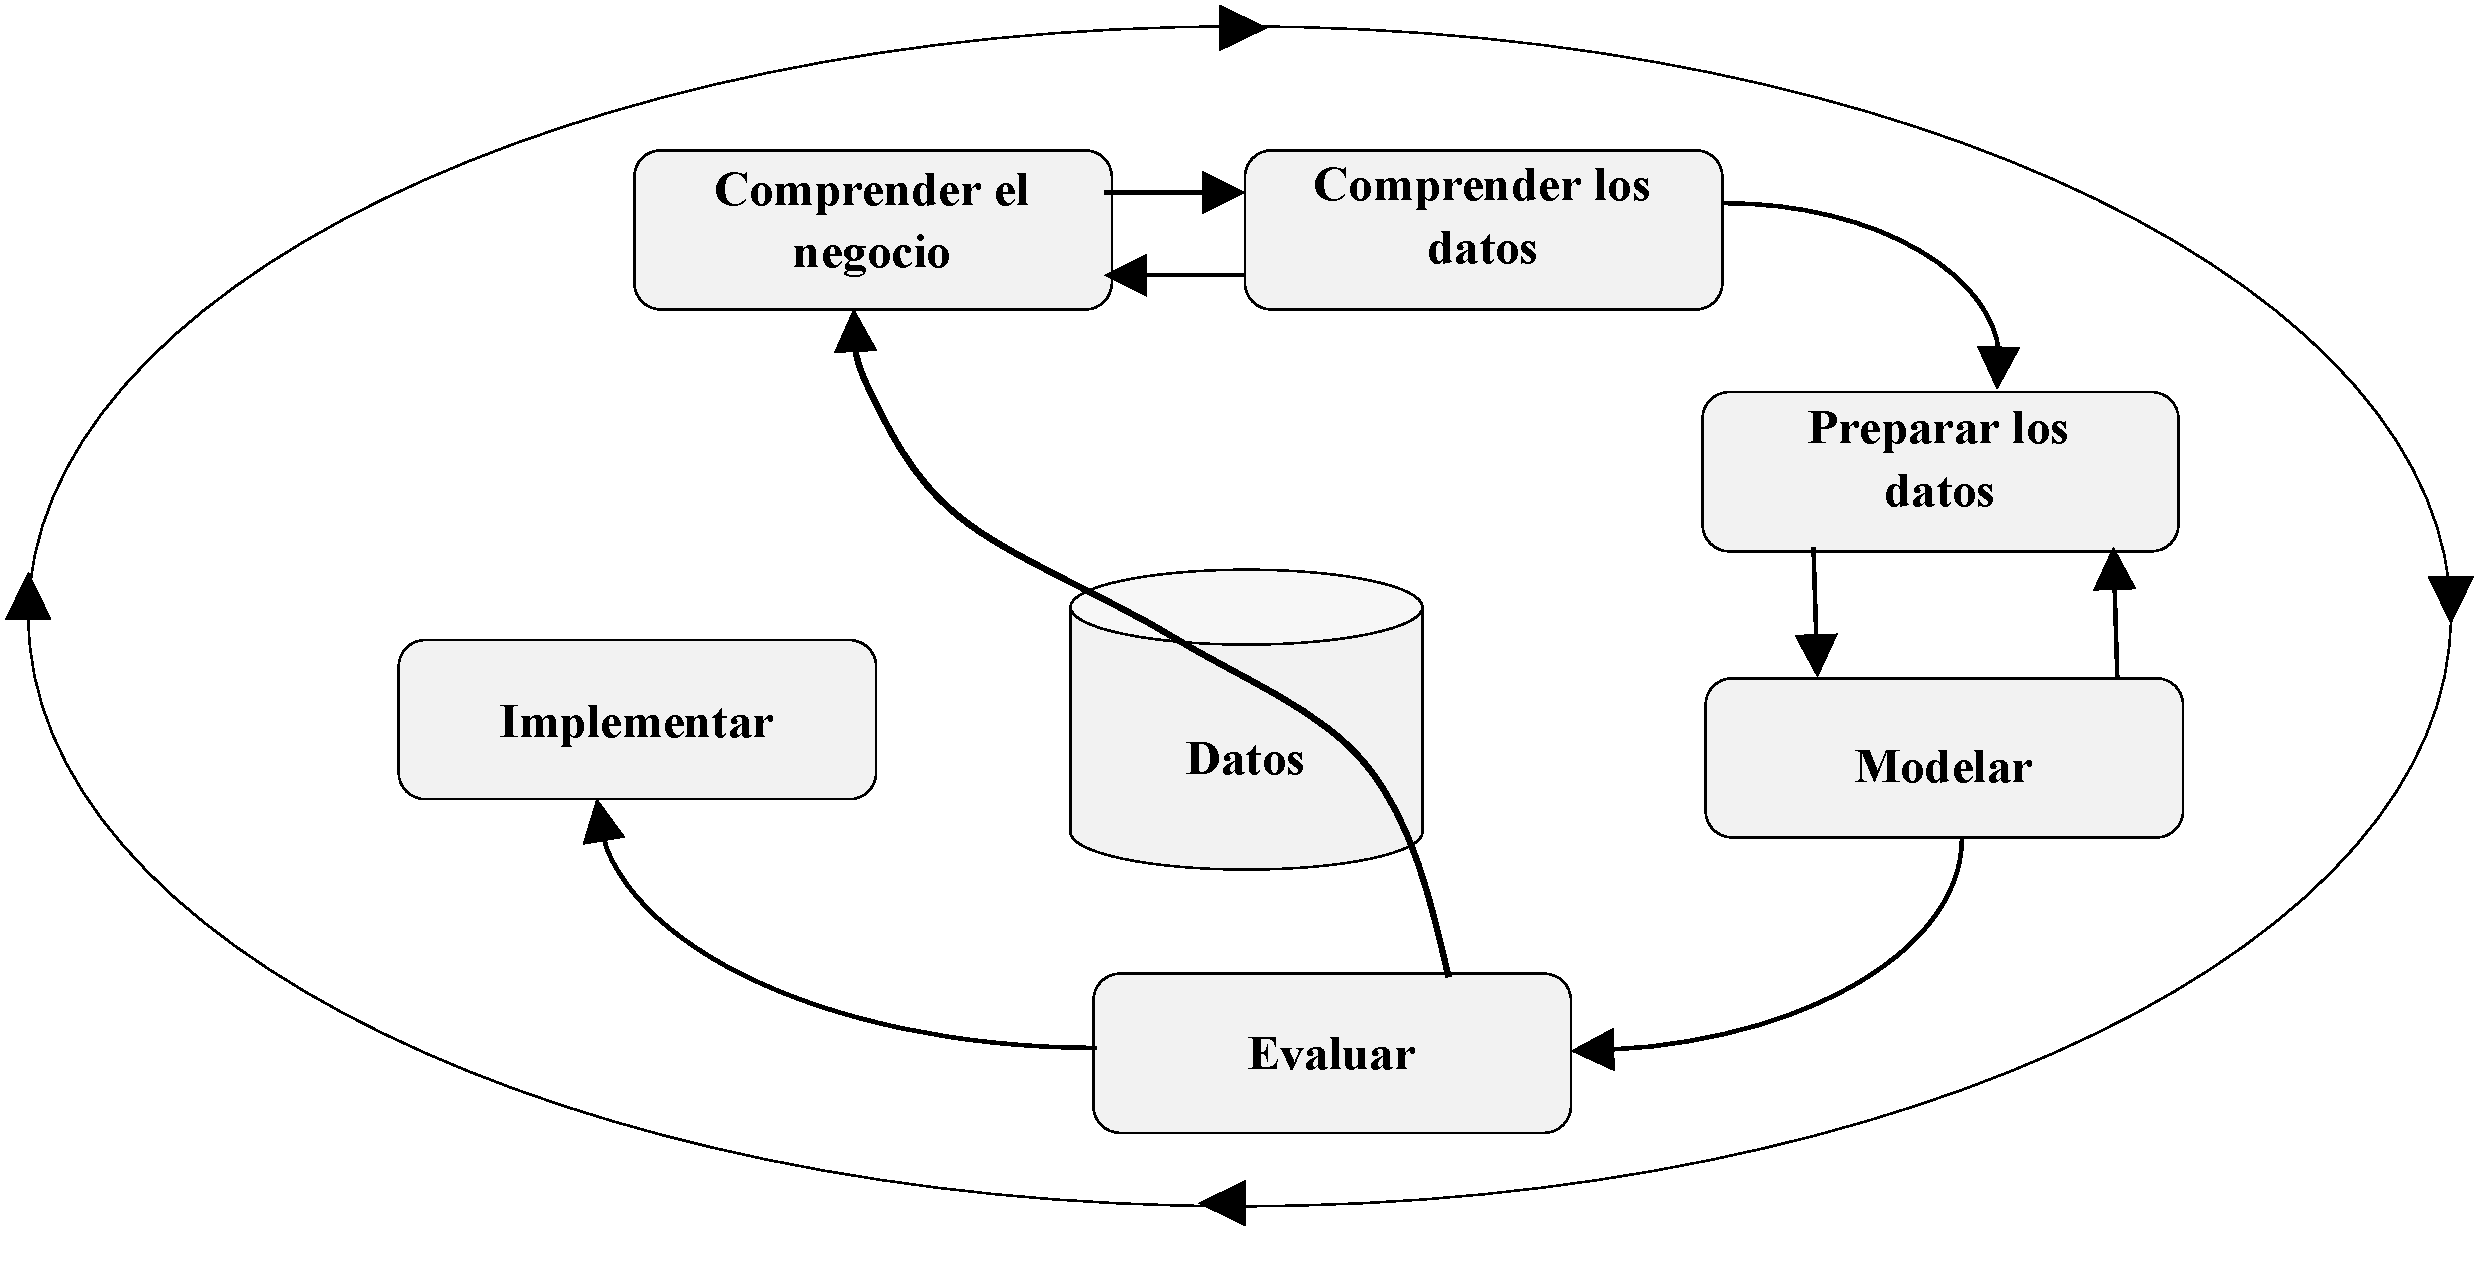
\includegraphics[width=0.75\textwidth]{images/fig-001.pdf}
 \caption{Modelo de proceso CRISP-DM }
 \label{Figura 1}
 \source{\cite{Wirth2000}}
\end{figure}

\subsection{Comprender el negocio}\label{sec-conduta}

Se definen los criterios de éxito cualitativos o cuantitativos. Luego, se evalúa el estado de la situación antes de iniciar el proceso de minería de datos, que involucra el nivel de conocimiento disponible acerca del problema. Se analiza la cantidad de datos disponibles y requerida, la relación costo beneficio, entre otros, para definir los requisitos del problema, tanto en términos del negocio como de minería de datos. Y, finalmente, se genera el plan del proyecto, el cual describe los pasos a seguir y las técnicas a emplear.

\subsection{Comprender los datos}\label{sec-fmt-manuscrito}

La segunda fase (\cref{Figura 2}) se inicia con la recopilación de los datos iniciales, extraídos desde una plataforma informática. Además, para establecer las variables que impactan en la deserción, se considera previamente lo expuesto en \cite{Cabrera2006} (ver \Cref{Tabla 2}).

\begin{figure}[htbp]
 \centering
 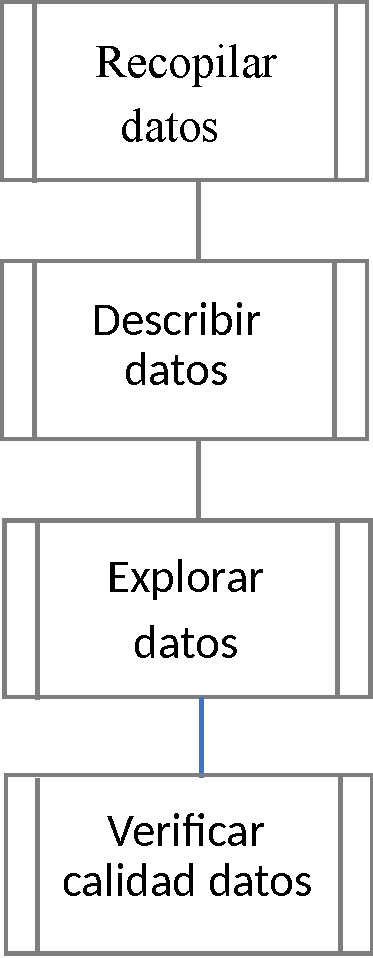
\includegraphics[width=0.25\textwidth]{images/fig-002.pdf}
 \caption{Actividades de la etapa de comprensión de los datos}
 \label{Figura 2}
 \source{Elaboración propia  en base a \cite{Wirth2000}}
\end{figure}

\begin{table}[htpb]
  \caption{Lista potencial de factores considerados.}
  \label{Tabla 2}
  \centering
  \begin{tabular}{ll}
  \toprule
  Autor & Factores considerados\\
  \midrule
  \multirow{3}{5cm}{\cite{Lujan1981}}  &
  Políticos\\
  & Económicos\\
  & Sociales\\
  \cmidrule{1-2}
  \multirow{3}{5cm}{\cite{Ryan2003}; \cite{Wasserman2001}; \cite{Kirton2000}; \textcite{Yip2019}}  &
  Personales\\
  & Institucionales\\
  & Sociales\\
  & Psicológicos\\
  & Educacionales\\
  \bottomrule
  \end{tabular}
  \source{Elaboración propia}
\end{table}

Luego, mediante entrevistas, los factores se validan por expertos internos y externos a la Institución, cuya opinión acotó a cuatro factores: económicos, educacionales, personales y sociales.

En la descripción de las variables se dividen en sociodemográficas y de comportamiento. Las seis variables sociodemográficas consideran el año y la edad al ingresar a la Institución (Año proceso y Edad al ingreso), género (Sexo), sede (Sede), jornada diurna o vespertina que asiste (Jornada) y país donde realizó sus estudios previos (País).

Las diez variables de comportamiento se subdividen en dos grupos, las de comportamiento previo y posterior al ingreso a estudiar, como se describe en la \Cref{Tabla 3}.

\begin{table}[htpb]
  \caption{Variables de comportamiento previo y posterior al ingreso a estudiar.}
  \label{Tabla 3}
  \centering
  \begin{tabular}{p{6,5cm}p{6,5cm}}
  \toprule
  Variables preingreso & Variables posingreso\\
  \midrule
  NEM - factor de selección para ingresar a ES, correspondiente al promedio de notas de la enseñanza media (CINE 3 y 4) \cite{UNESCOInstituteforStatistics2012}. & Asignaturas inscritas – número de materias inscritas en el año, considerando los dos semestres.\\
  \cmidrule{1-2}
  Facultad - área del conocimiento que contiene a la carrera elegida por el estudiante. & Asignaturas aprobadas – número de materias aprobadas en el primer año, considerando los dos semestres.\\
  \cmidrule{1-2}
  Puntaje Ranking - factor de selección para ingresar a ES, cuyo puntaje representa el lugar que ocupa el puntaje NEM del estudiante en relación con el promedio de notas de todos los alumnos de su contexto educativo de las tres generaciones anteriores a la suya. & Asistencia – resultado de la división del número de horas asistidas y la cantidad total de horas de clase correspondiente a las asignaturas inscritas en el primer año, expresado como porcentaje.\\
  \cmidrule{1-2}
  Promedio puntaje Lenguaje y Matemática - factor de selección para ingresar a ES, definido como el puntaje promedio entre los resultados obtenidos en las pruebas de Lenguaje y Comunicación, y Matemática. & Abandono - variable objetivo que refleja la situación de seguir estudiando o no durante el segundo año.\\
  \cmidrule{1-2}
  Puntaje Ciencias o Historia - factor de selección para ingresar a ES, que equivale al puntaje alcanzado en la prueba de Ciencias o en la de Historia, Geografía y Ciencias Sociales. & \\
  \cmidrule{1-2}
  Vía admisión a estudios superiores – representa el modo de ingreso del estudiante a la educación superior. & \\
  \bottomrule
  \end{tabular}
  \source{Elaboración propia}
\end{table}

Una tercera actividad es la exploración de los datos. Se analizan las distribuciones para así examinar subconjuntos de datos que representan las subpoblaciones a caracterizar.

Preliminarmente, desde el ámbito demográfico, se encontró que a medida que aumenta la edad, disminuye la frecuencia de estudiantes en el rango etario. Las frecuencias relativas mostraron que la mayoría, un 61~\%, son hombres. Casi la totalidad, un 99,6~\%, realizaron sus estudios previos en establecimientos nacionales y no en el extranjero. Un 86~\%, están inscritos en jornada diurna y el resto en vespertina. Y, por último, un 86~\%, inició su carrera desde un principio, es decir, no se realizó alguna convalidación u homologación de asignaturas.

Desde una perspectiva institucional, las sedes con mayor captación de alumnos son La Serena y Santiago, con un 34~\% y 28~\% respectivamente. Y las facultades con mayor ingreso son Ciencias de la Salud (30~\%) y Educación (20~\%), que suman la mitad del total de casos estudiados (las facultades con menor cantidad de casos son la de Odontología y Ciencias Agropecuarias).

En el ámbito académico, existen estudiantes que provienen de colegios más vulnerables, que optan por el ingreso vía ranking, y alcanzan el 36~\%. La mayoría de las notas NEM se concentran entre 5,0 y 6,0, y representan el 73~\% del total. El 37~\% de los casos estudiados abandonó.

Como cuarta actividad, se verifica la calidad de los datos, es decir, revisar que estén completos y sin errores o valores fuera de rango. Por un lado, se descubren registros con valores inconsistentes, principalmente por ausencia de datos en NEM y puntajes de prueba (lenguaje, matemática, ciencia e historia), alumnos sin asignaturas inscritas, entre otros. Además, se identifican registros con estudiantes de la sede Concepción y/o la Facultad de Arquitectura, cuyos conflictos administrativos pueden generar un sesgo en el análisis.

\subsection{Preparar los datos}\label{sec-formato}

Se integran datos mediante cruce de información (\cref{Figura 3}). Luego, se eliminan todos los registros inconsistentes, identificados en la etapa anterior. Así, se obtiene una base de 6299 casos de un total de 9523, que implica una limpieza del 34~\% de los datos. La tercera tarea es la construcción de los datos. Para permitir una mejor representación de la información, se expresa en porcentaje la variable Asignaturas aprobadas, a partir del cociente entre asignaturas aprobadas e inscritas; además, se generó la variable dicotómica Abandono, obtenida de la misma base, que verifica si el alumno se matriculó o no en el año posterior a su ingreso.

\begin{figure}[htbp]
  \centering
  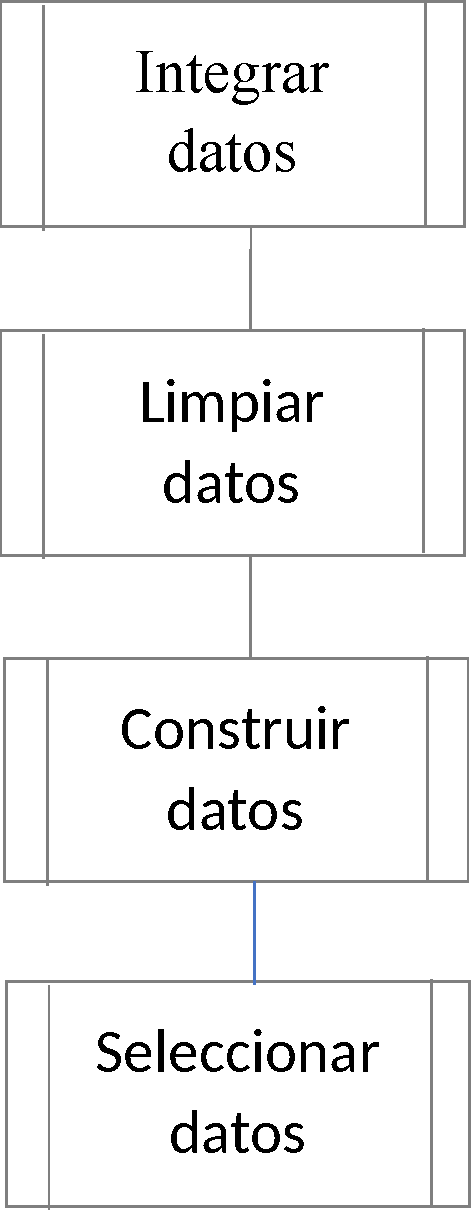
\includegraphics[width=0.25\textwidth]{images/fig-003.pdf}
  \caption{Actividades de la etapa de preparación de los datos}
  \label{Figura 3}
  \source{Elaboración propia  en base a \cite{Wirth2000}}
\end{figure}

Dicho lo anterior, las variables se reducen a trece, descartándose Año proceso, Sexo y Jornada, porque entre sus posibles valores no se puede atribuir mayor importancia a uno por sobre otro respecto al fenómeno de deserción. Además, se renombran y codifican las variables cualitativas factibles de jerarquizar, ya que el programa XLSTAT \cite{Addinsoft} no reconoce este tipo de variables. Se aplica una codificación entera a Riesgo país de procedencia (antes llamada Nacionalidad), Riesgo facultad (antes llamada Facultad), Riesgo sede (antes llamada Sede), Riesgo ranking (antes llamada Puntaje Ranking) según \cite{Donoso2007a}, Riesgo vía admisión (antes llamada Vía admisión) según \cite{Donoso2007a}, y Abandono. Finalmente, se aplican dos métodos para seleccionar las variables más predominantes en la deserción. En primera instancia se realiza un análisis de correlación, con el cual se obtienen las variables más correlacionadas con la deserción \cite{Hernandez2018}.

Para reforzar la selección de variables se lleva a cabo el ACP \cite{Fenyes2021}. Así, se obtienen los valores propios de la matriz de correlaciones, que corresponden a las componentes principales, combinaciones lineales de las variables estandarizadas. Se trabajó, además, con el gráfico de sedimentación y el círculo de correlaciones para determinar los factores a considerar.

\subsection{Modelar}

A partir de las variables más correlacionadas con la deserción, se definen diversos perfiles de estudiante, agrupados según la similitud de sus comportamientos. En un primer paso (\cref{Figura 4}), se propone aplicar CJA, definir las distintas clases o grupos, analizar estadísticamente los resultados obtenidos para establecer las variables que explican el abandono y así, definir los perfiles de estudiantes \cite{Antonenko2012}.

\begin{figure}[htbp]
  \centering
  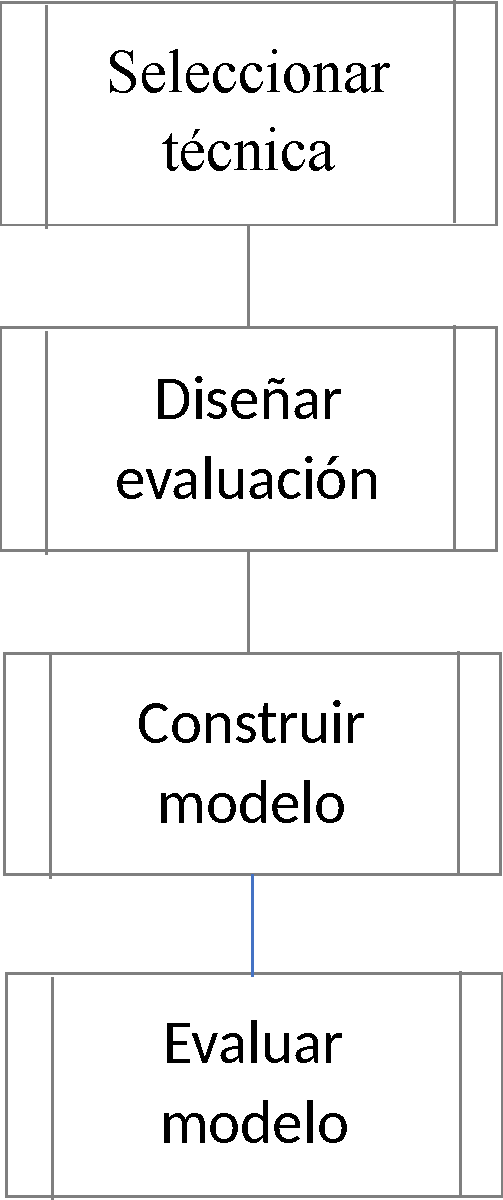
\includegraphics[width=0.25\textwidth]{images/fig-004.pdf}
  \caption{Actividades de la etapa de modelación}
  \label{Figura 4}
  \source{Elaboración propia  en base a \cite{Wirth2000}}
\end{figure}

Para determinar la medida de disimilaridad se utilizó el método de Ward \cite{Vijaya2019}. Consiste en unir los dos clúster para los cuales se tenga el menor incremento en el valor total de la suma de los cuadrados de las diferencias, dentro de cada clúster, de cada individuo al centroide del clúster. Así, se obtiene la ventaja de no dejar grupos que tengan pocos elementos, se facilita la formación de clúster más compactos y de tamaño relativamente similar, y se minimiza la pérdida de información en el proceso de organización de conglomerados \cite{Tseng2016}.

Para detectar las diferencias entre clases se obtuvo el comportamiento promedio según variables de entrada. Para verificar si la media aritmética de los factores es una herramienta adecuada de comparación entre clases, se calcula la moda, la mediana y la desviación estándar para cada factor en cada clase. Para evaluar la dispersión en cada variable de entrada seleccionada se utiliza el gráfico de caja y bigote. De esta manera se puede observar en cuáles clases y en qué cuartil se presenta una oportunidad de hacer seguimiento y mejorar los índices obtenidos, al indagar en las posibles causas que originan esta situación.

Los perfiles obtenidos a partir del CJA \cite{Buritica2019}, según el comportamiento de las variables definidas como de mayor preponderancia, se validan o refutan. Se busca identificar y definir las principales reglas de asociación de los estudiantes de cada grupo, en relación con las variables en estudio y el fenómeno de deserción. Para esto se utiliza el método de conjuntos aproximados con un enfoque basado en dominancia (DRSA) \cite{Bouzayane2017,Greco1999,Greco2002a}, el cual aplica a problemas de decisión multicriterio basado en relaciones de dominancia, para obtener la aproximación de una relación de preferencia. El software 4eMka2 \cite{Greco1999,LaboratoryofIntelligentDecisionSupportSystemsIDSS} entrega diversas reglas de decisión basadas en condiciones y los siguientes criterios de medición de las reglas: coverage, support y strength (razón porcentual entre support y coverage que indica la consistencia). Así, se escogen las reglas de mayor relevancia respecto a los valores alcanzados en estos índices, al considerar como variable decisional el hecho de abandonar o no.

Para obtener reglas confiables se realizó el mismo análisis anterior por clases, pero se estudian de manera independiente las reglas obtenidas para los alumnos que abandonan y quienes no. Luego, se resumen las reglas según mayor consistencia presentada, independientemente de la clase de pertenencia. Con esto se obtienen variables que permiten explicar transversalmente el fenómeno de deserción para el universo de estudiantes en cada una de las clases definidas.

Finalmente, se obtienen las reglas de asociación, con el número de clase del estudiante como variable decisional, sin considerar la variable Abandono. Así, se obtienen las principales reglas que rigen para cada clase, además de verificar la complementariedad existente entre los distintos grupos. Con el análisis de clúster, entonces, se obtienen las variables que mayor incidencia podrían tener sobre la deserción, y si tienen la incidencia suficiente como para explicar este fenómeno por sí solas.

\subsection{Evaluar}

A partir de las variables más correlacionadas con el abandono y de los perfiles de estudiantes, se generan dos propuestas de mejora al modelo de gestión estudiantil con el fin de mitigar la deserción y fomentar la retención.

\section{Resultados y discusión}\label{sec-modelo}

En la preparación de los datos, tercera etapa del proceso CRISP-DM, se obtienen los resultados del análisis de correlación (\Cref{Tabla 4}), del cual solo siete variables de las trece consideradas presentan un coeficiente de correlación mayor a 0,1 \cite{Hernandez2018}, descartándose las otras seis.

\begin{table}[htpb]
    \caption{Coeficiente de correlación entre las 12 variables consideradas y la deserción.}
    \label{Tabla 4}
    \centering
    \begin{tabular}{ll}
    \toprule
    Variables de entrada & Abandono (Sí/No)\\
    \midrule
    Edad al ingreso & -0,002\\
    Riesgo país de procedencia & 0,009\\
    Riesgo facultad & 0,062\\
    Riesgo sede & -0,006\\
    NEM & -0,121\\
    Riesgo Ranking & -0,139\\
    Promedio puntaje Lenguaje y Matemática & -0,114\\
    Puntaje Ciencias o Historia & -0,104\\
    Asignaturas inscritas & -0,436\\
    Asignaturas aprobadas & -0,598\\
    Asistencia & -0,476\\
    Riesgo vía admisión & -0,046\\
    \bottomrule
    \end{tabular}
    \source{Elaboración propia}
\end{table}

Del ACP aplicado a las trece variables originales se obtiene el gráfico de sedimentación (\cref{Figura 5}) y el círculo de correlaciones (\cref{Figura 6}). En el primero se observa que las dos primeras componentes acumulan el 39~\% de la variabilidad, que puede considerarse en un principio un nivel de representación aceptable dada la tasa de acumulación de variabilidad menor a partir de la tercera componente.

\begin{figure}[htbp]
 \centering
 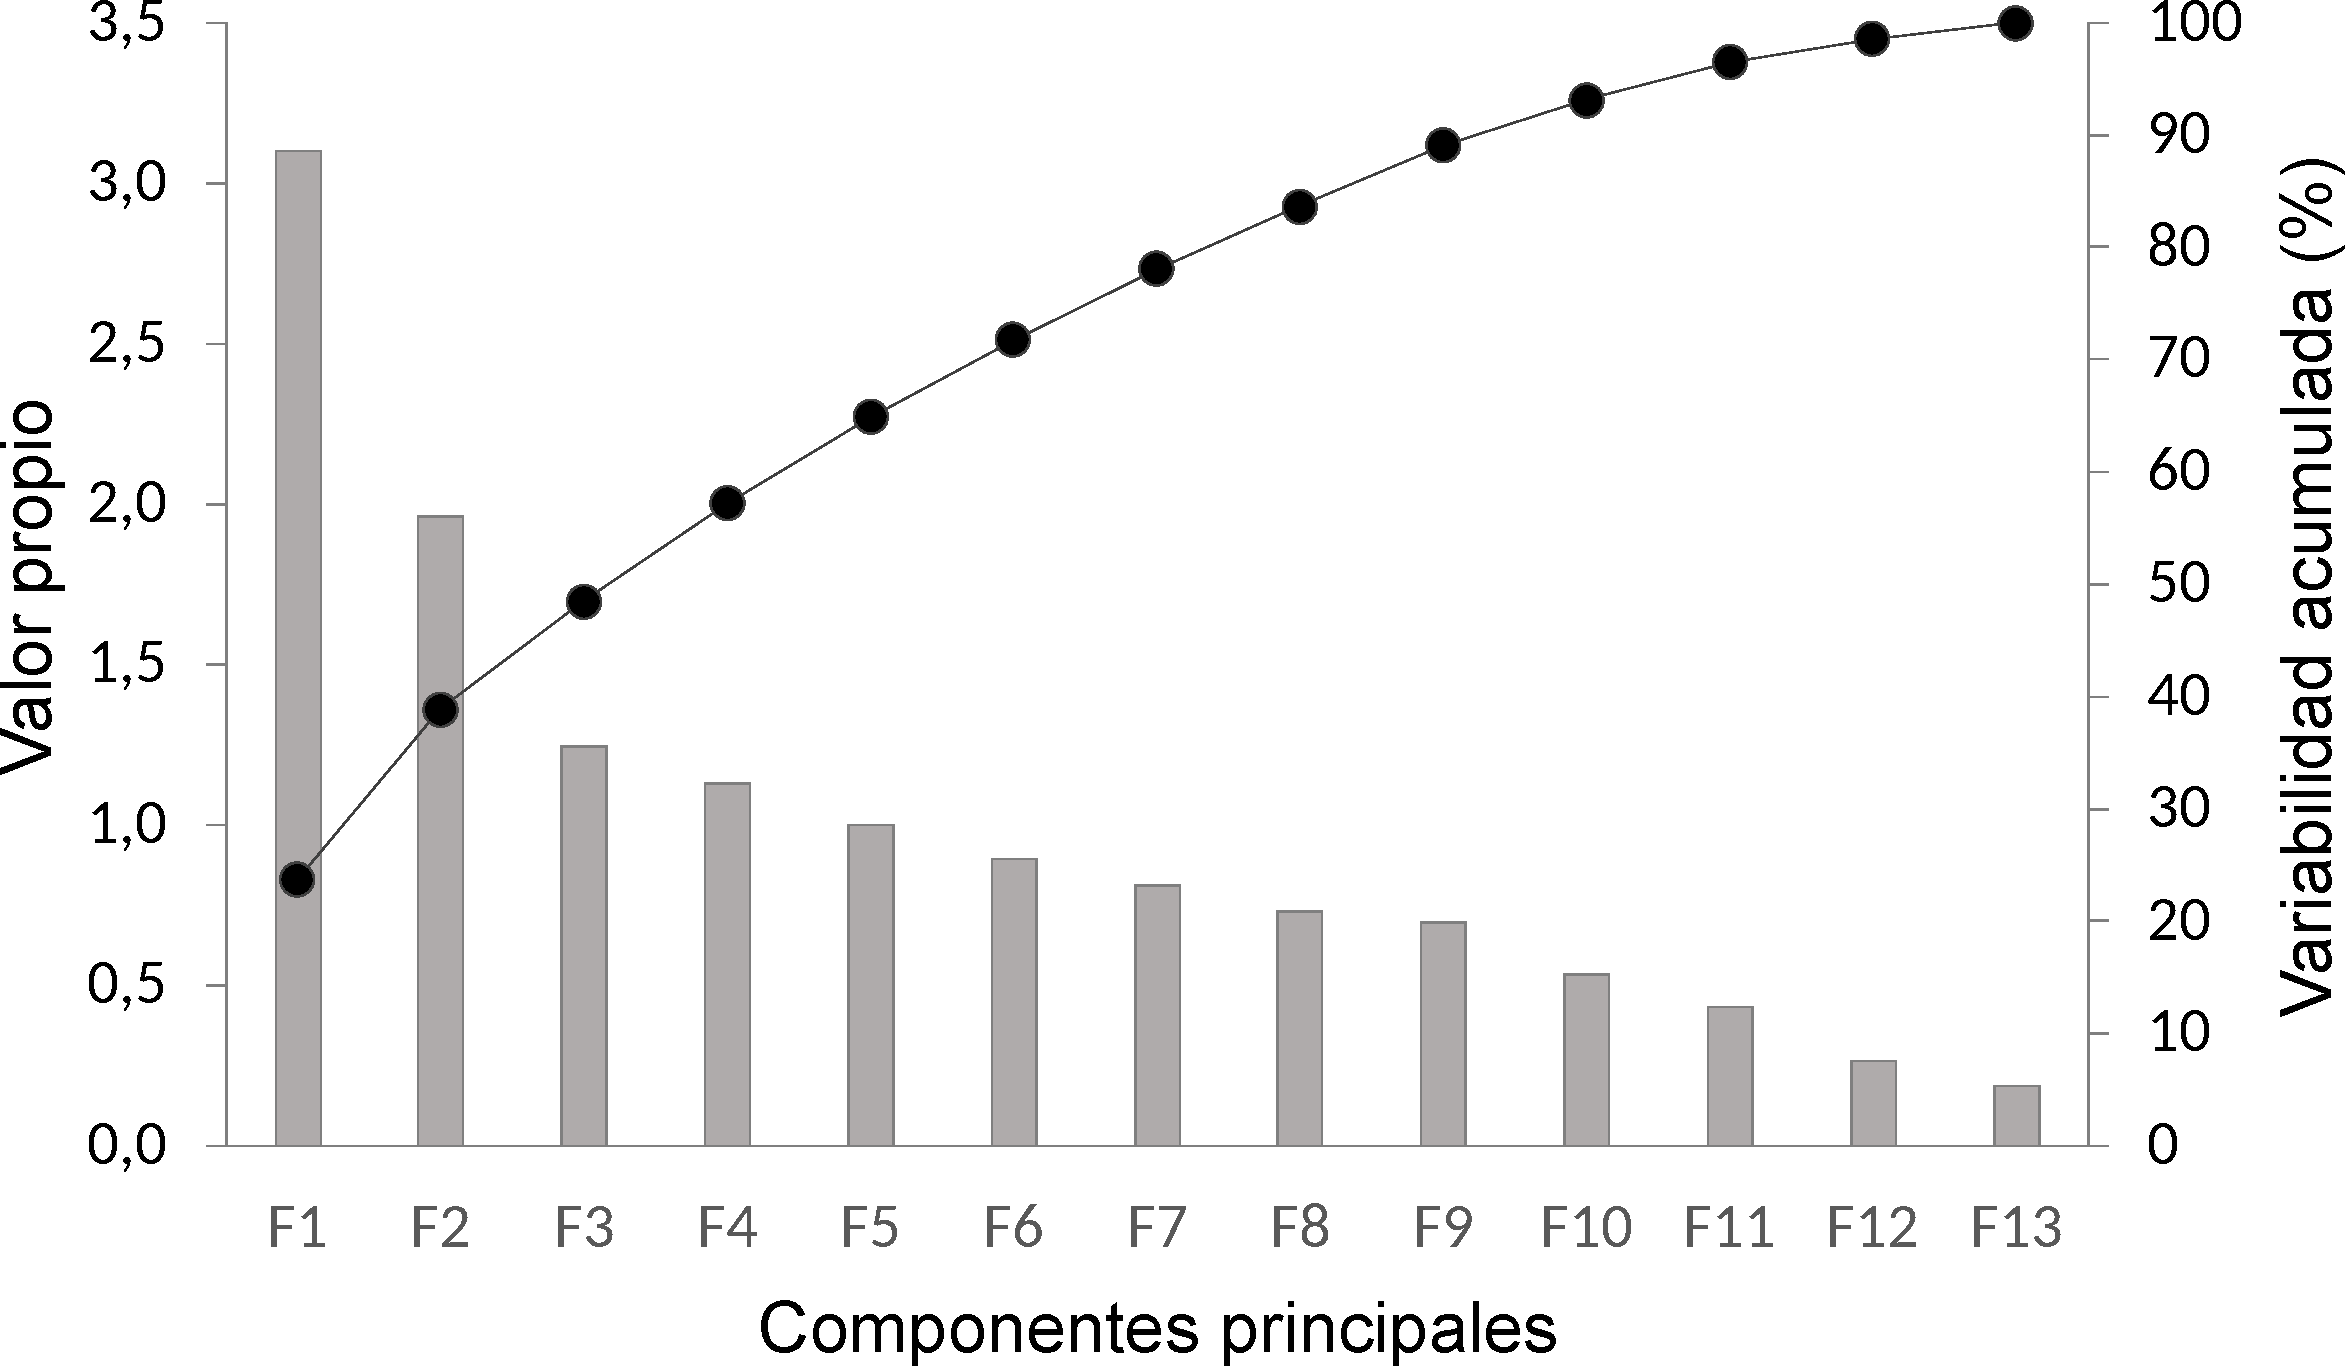
\includegraphics[width=0.75\textwidth]{images/fig-005.pdf}
 \caption{Valores propios y porcentaje de la inercia explicada, de las componentes principales}
 \label{Figura 5}
 \source{Elaboración propia.}
\end{figure}

\begin{figure}[htbp]
 \centering
 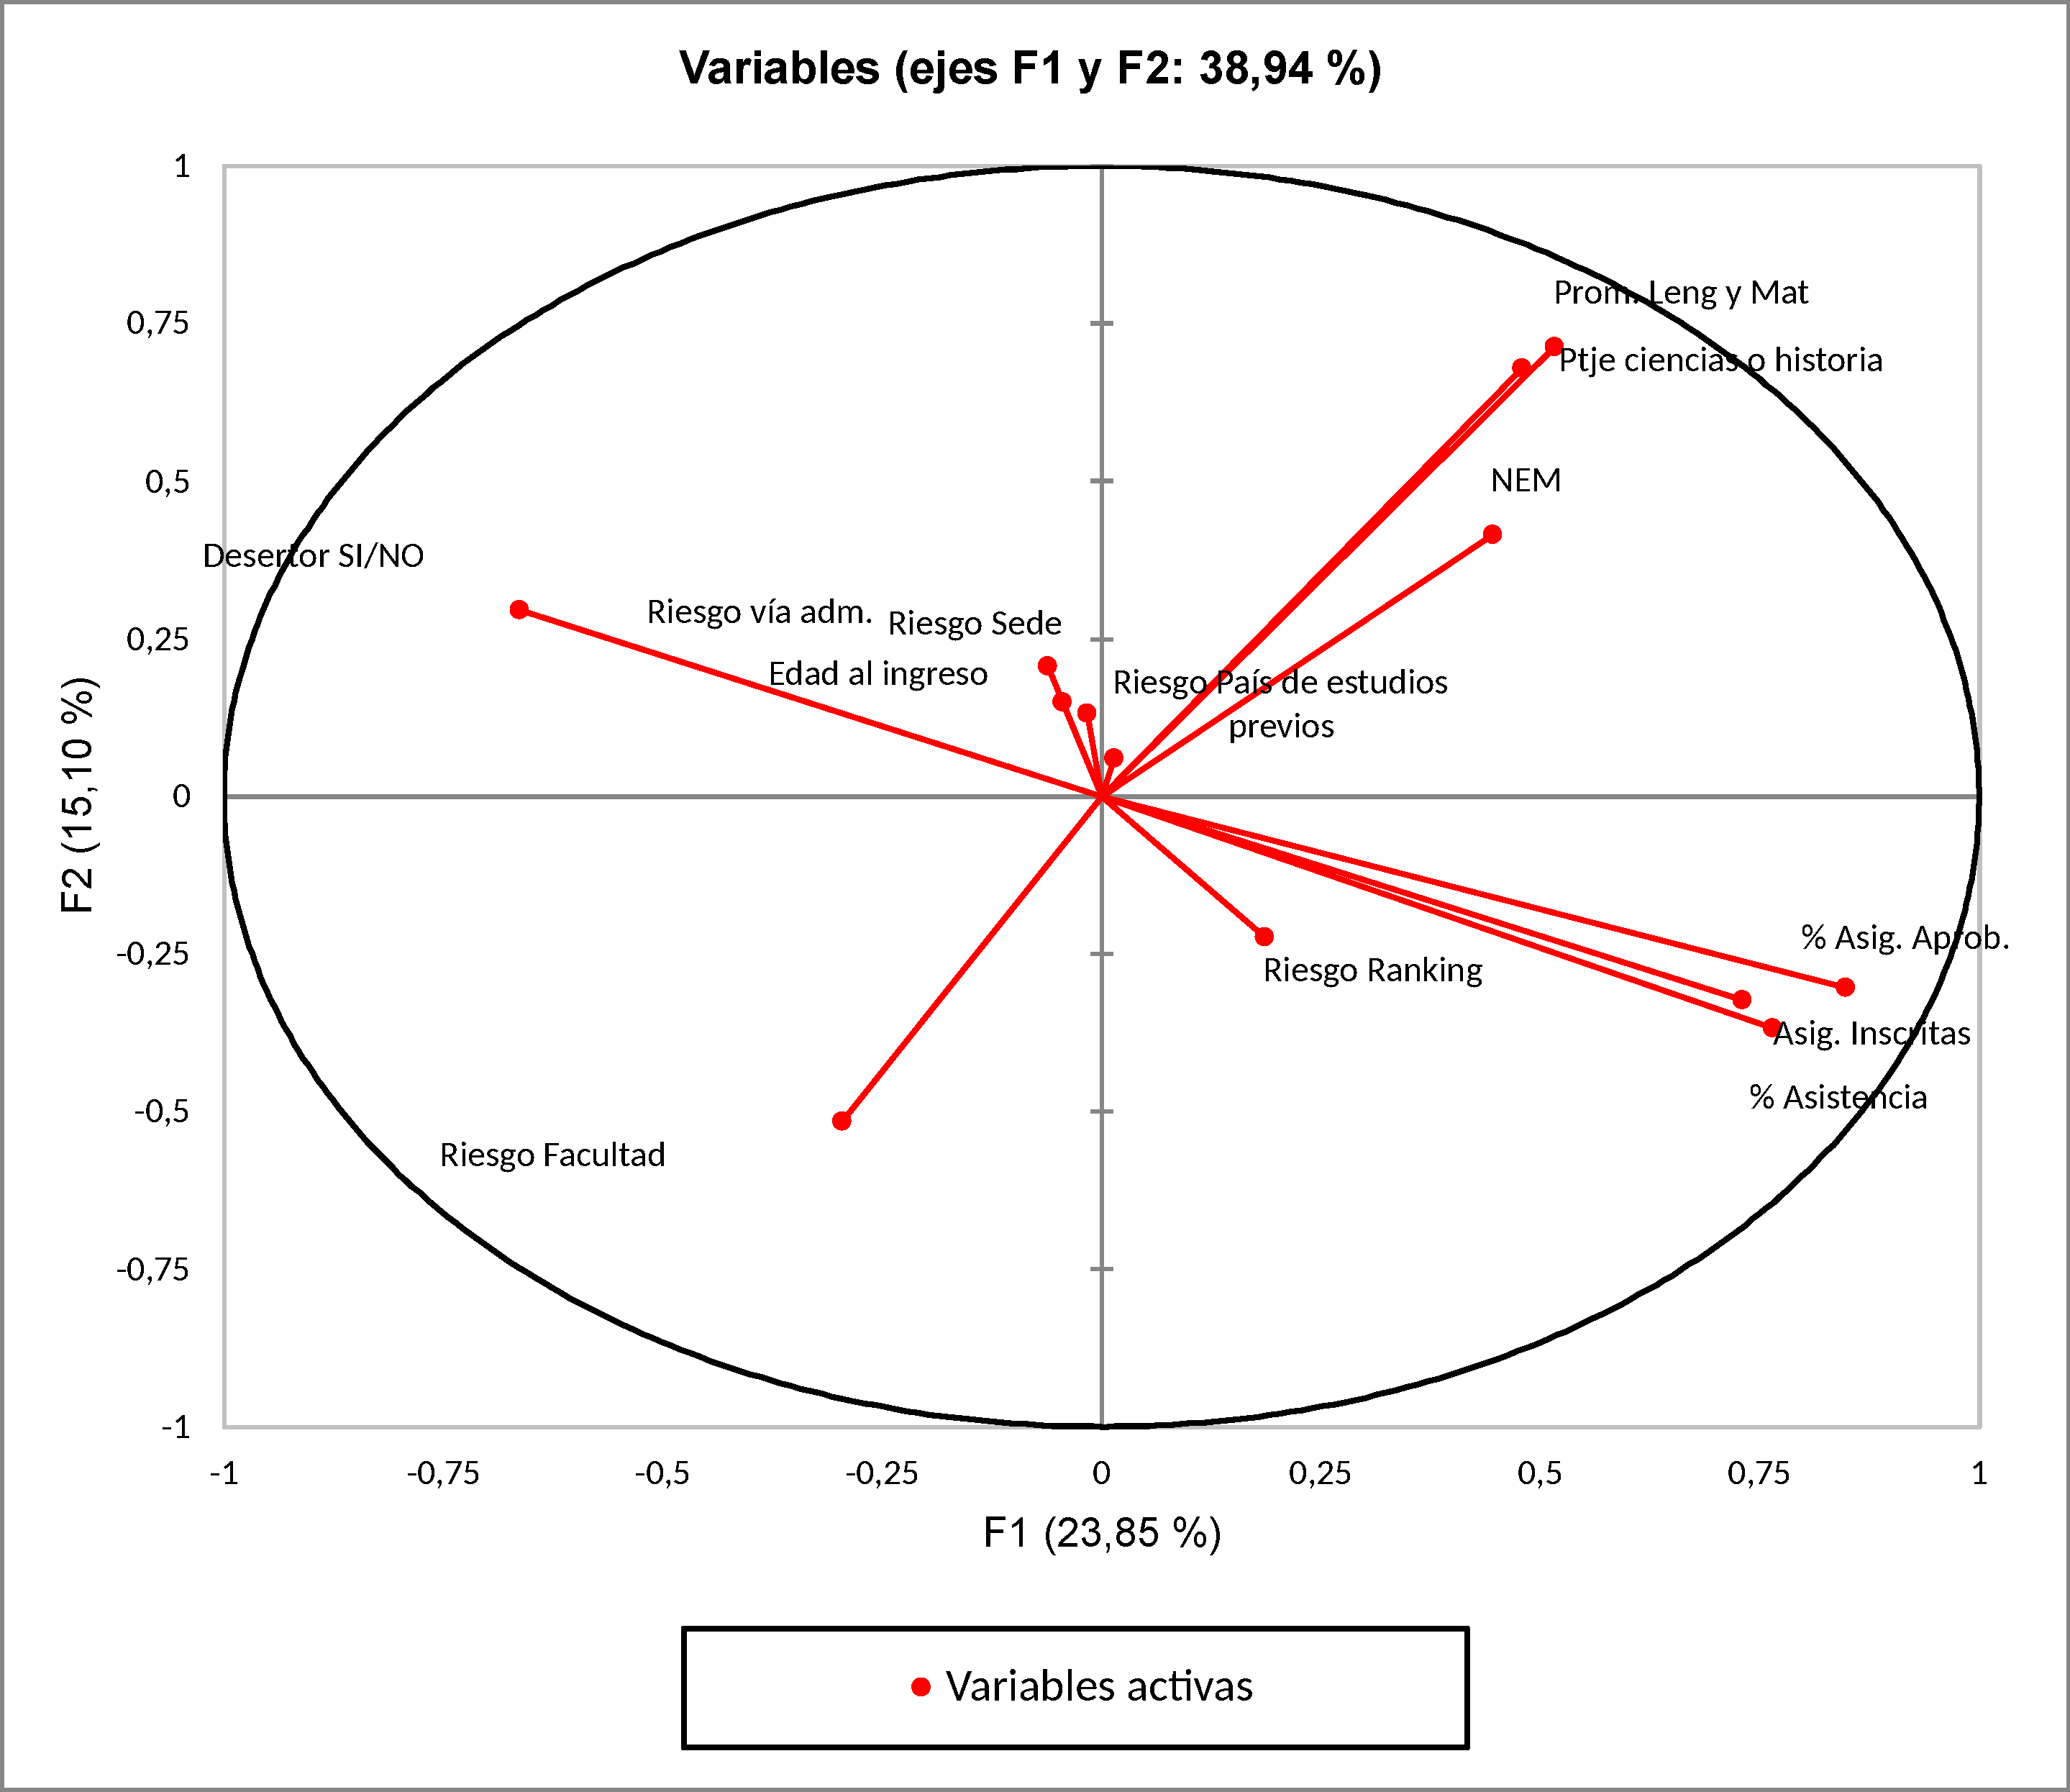
\includegraphics[width=0.75\textwidth]{images/fig-006.pdf}
 \caption{Círculo de correlaciones para las trece variables}
 \label{Figura 6}
 \source{Elaboración propia.}
\end{figure}

El círculo de correlaciones muestra que solo las variables académicas posingreso (Asignaturas aprobadas, Asignaturas inscritas y Asistencia) están fuertemente correlacionadas con la deserción. De las variables preingreso, cuatro no están correlacionadas (Promedio puntaje Lenguaje y Matemática, Puntaje Ciencia o Historia, NEM, Riesgo facultad) y solo Riesgo Ranking presenta cierta correlación. Para el resto de las variables esta gráfica no permite generar inferencias. Por esta razón, se trabaja con las siete variables resultantes del análisis de correlación.

A través de CJA se obtuvieron cuatro grupos o clases, cuyas características permiten su diferenciación (\Cref{Tabla 5}). Se observa que a medida que un grupo presenta una mayor deserción promedio, menor es el valor promedio en las variables de entrada, excepto para la variable descartada Riesgo Ranking. Aun así, el grupo que presenta la mayor tendencia al abandono (grupo 3) no alcanza a presentarlo en la mayoría de los estudiantes (43,7~\%).

\begin{table}[htbp]
    \caption{Promedio de variables para los 4 grupos obtenidos, ordenados por variable Abandono.}
    \label{Tabla 5}
    \centering
    \begin{tabular}{lllll}
    \toprule
    Variable &
    \multicolumn{4}{c}{Clase}\\
    & 4 & 1 & 2 & 3\\
    \midrule
    NEM & 5,98 & 5,62 & 5,47 & 5,35\\
    Riesgo Ranking & 1,44 & 1,27 & 1,34 & 1,41\\
    Promedio puntaje Lenguaje y Matemática & 631 & 541 & 467 & 392\\
    Puntaje Ciencias o Historia & 631 & 560 & 481 & 373\\
    Asignaturas inscritas & 12,8 & 11,4 & 10,9 & 10,6\\
    Asignaturas aprobadas & 86,7~\% & 79,7~\% & 70,5~\% & 62,7~\%\\
    Asistencia & 85,4~\% & 82,2~\% & 80,2~\% & 78,0~\%\\
    Abandono & 0,250 & 0,314 & 0,371 & 0,437\\
    \bottomrule
    \end{tabular}
    \source{Elaboración propia}
\end{table}

Para llegar a resultados más concluyentes, se profundizó el análisis anterior dividiendo los grupos en subgrupos de estudiantes que abandonan y los que no (\Cref{Tabla 6}).

\begin{table}[htbp]
    \caption{Promedio de variables de entrada para los 4 grupos obtenidos, subdivididos según condición de abandono y ordenados por variable Abandono.}
    \label{Tabla 6}
    \centering
    \begin{tabular}{lllllllll}
    \toprule
    Variable & \multicolumn{8}{c}{Abandono}\\
     &
    \multicolumn{2}{c}{Clase 4} &
    \multicolumn{2}{c}{Clase 1} &
    \multicolumn{2}{c}{Clase 2} &
    \multicolumn{2}{c}{Clase 3}\\
     &
     No & Sí & No & Sí & No & Sí & No & Sí\\
     \midrule
     NEM & 6,01 & 5,91 & 5,63 & 5,62 & 5,51 & 5,42 & 5,39 & 5,30\\
     Promedio pje. L. y M. & 631 & 630 & 541 & 540 & 468 & 466 & 394 & 388\\
     Puntaje Cs. o Hist. &	632	& 629 &	560 & 561 & 482 & 480 & 373 & 372\\
     Asignaturas inscritas &	13,5 & 10,6 & 12,0 & 10,1 & 12,0 & 9,0 & 12,0 & 8,8\\
     Asignaturas aprobadas & 0,94 & 0,64 & 0,89 & 0,59 & 0,86 & 0,43 & 0,83 & 0,37\\
     Asistencia & 88,85 & 74,97 & 85,71 & 74,58 & 86,38 & 69,74 & 85,96 & 67,61\\
     Abandono & 25,0~\% & 75,0~\% & 31,4~\% & 68,6~\% & 37,1~\% & 62,9~\% & 43,7~\% & 56,4~\%\\
     \bottomrule
    \end{tabular}
    \source{Elaboración propia}
\end{table}

Al comparar las variables de entrada por subgrupos y grupos que abandonan y quienes no, se puede inferir que:

Las variables NEM, Promedio puntaje Lenguaje y Matemática, y Puntaje Ciencias o Historia, no presentan una diferencia que permita explicar una tendencia al abandono en alguno de los grupos.

Las variables Asignaturas inscritas, Asignaturas aprobadas y Asistencia, muestran una clara diferencia entre subgrupos. En los estudiantes que abandonan, los valores promedio de estas variables son menores a quienes no lo hacen, independiente del grupo de pertenencia.

Con este resultado, se procedió a caracterizar los perfiles de los estudiantes, y se considera finalmente las variables Asignaturas aprobadas y Asistencia. Se descartó Asignaturas inscritas ya que al ingresar a un programa de estudio las asignaturas están predefinidas para el primer año, y en el caso que el alumno llegase a reprobar alguna, probablemente deba tomar menos asignaturas durante el segundo semestre, aspecto explicable con la variable Asignaturas aprobadas.

Para evaluar la dispersión de los datos en las dos variables de entrada seleccionadas se utilizó el gráfico caja y bigote. Se observan, para Asignaturas aprobadas (\cref{Figura 7}), rendimientos académicos decrecientes en los alumnos, reflejados en la mediana, con porcentajes de aprobación de 100~\%, 92~\%, 85~\% y 75~\%, correspondientes a las clases 4, 1, 2 y 3, respectivamente. Así, el menor rendimiento de las clases 1, 2 y 3 representa una oportunidad de mejora, en especial en los alumnos de la clase 3, que poseen mayor riesgo. En cuanto a la concentración de los datos, es mucho mayor para la clase 4, en la cual la mediana y el cuartil 3 coinciden con el valor máximo, y es mucho menor en la clase 3.

\begin{figure}[htbp]
 \centering
 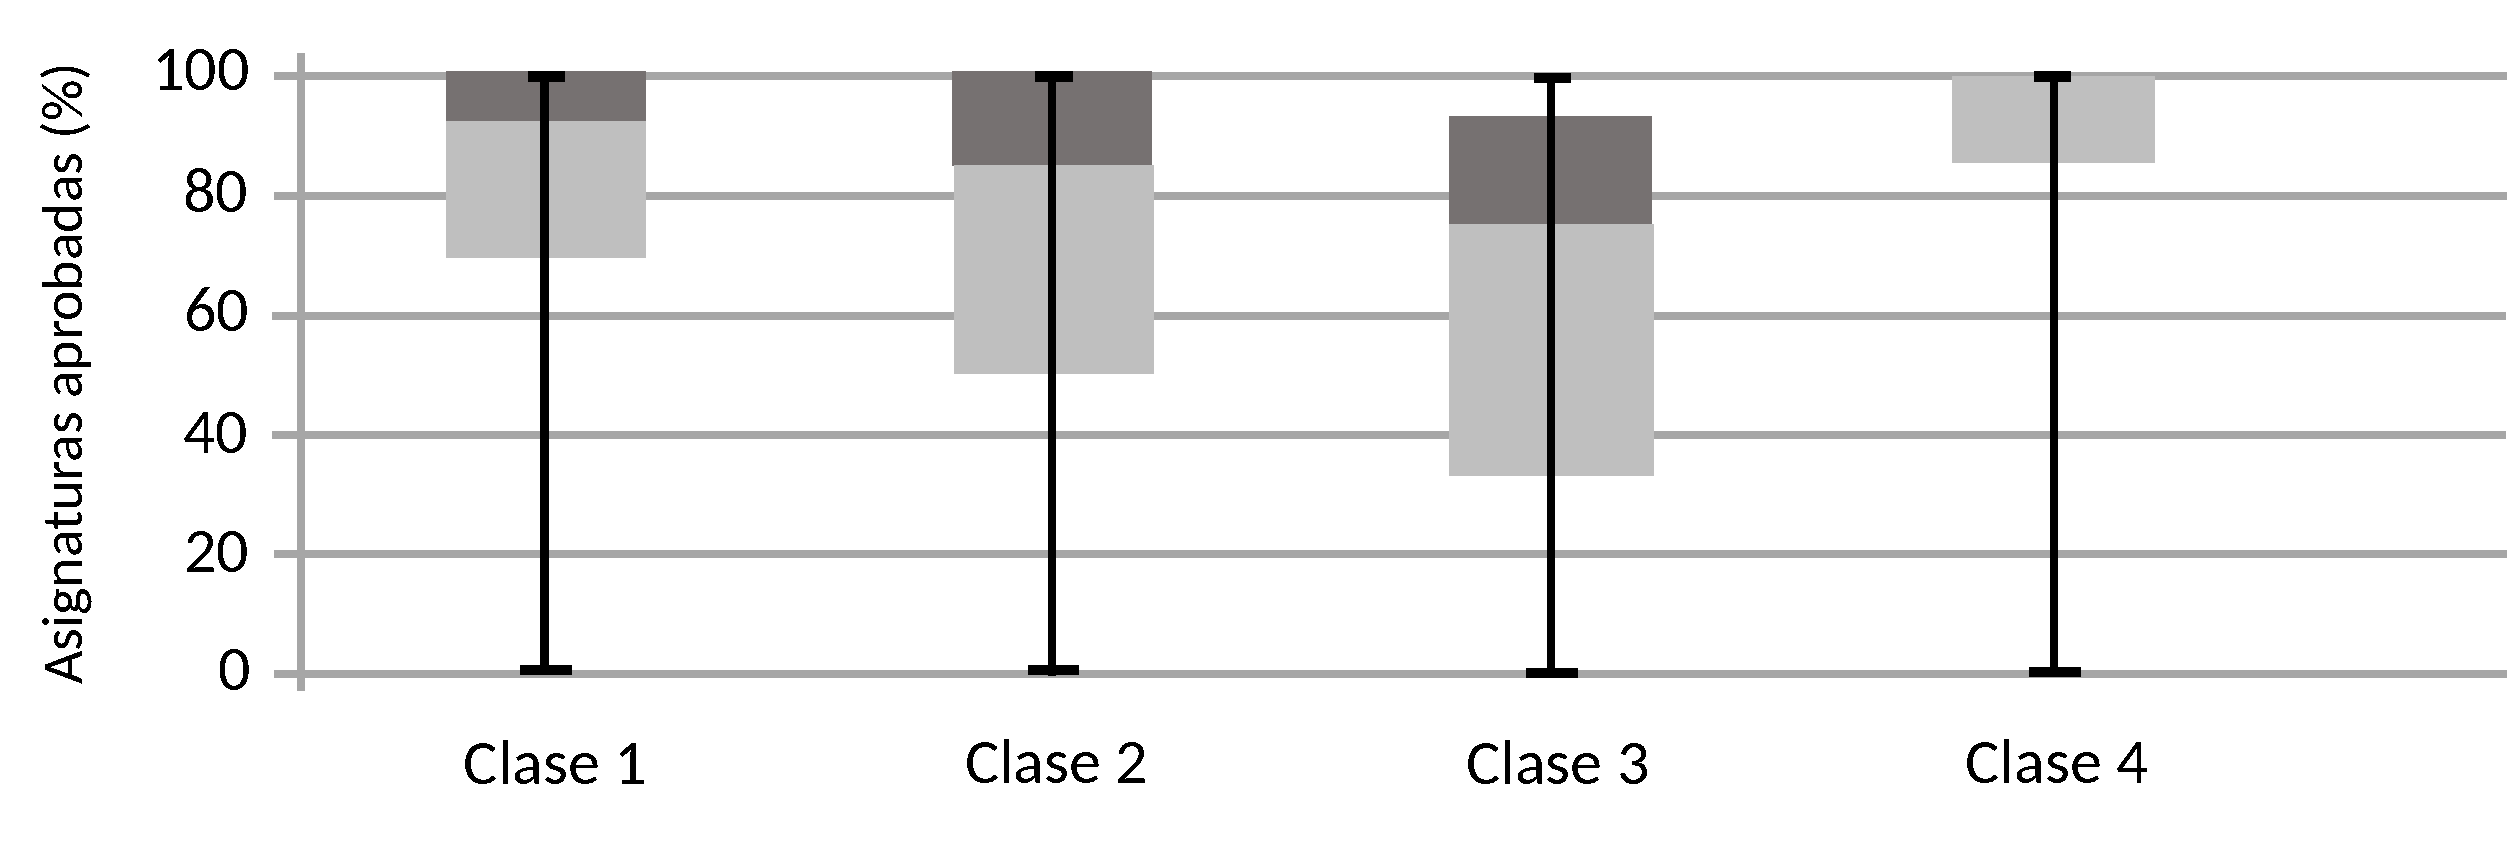
\includegraphics[width=0.75\textwidth]{images/fig-007.pdf}
 \caption{Caja y bigote de variable Asignaturas aprobadas, por cada grupo de estudiantes}
 \label{Figura 7}
 \source{Elaboración propia.}
\end{figure}

Para la variable Asistencia se observa la misma situación anterior, pero mucho más leve (\cref{Figura 8}). La asistencia tiende a decrecer con una mediana de 89~\%, 86~\%, 86~\% y 84~\% para los grupos 4, 1, 2 y 3, respectivamente. Así también, la dispersión tiende a aumentar, con un rango intercuartil de 9, 12, 13 y 15 puntos porcentuales para los grupos 4, 1, 2 y 3, respectivamente. De esta forma, en las cuatro clases se presenta una oportunidad de hacer seguimiento y mejorar los índices obtenidos, en especial con los alumnos del cuartil 1, en donde se deberán indagar las posibles causas de la baja asistencia.

\begin{figure}[htbp]
 \centering
 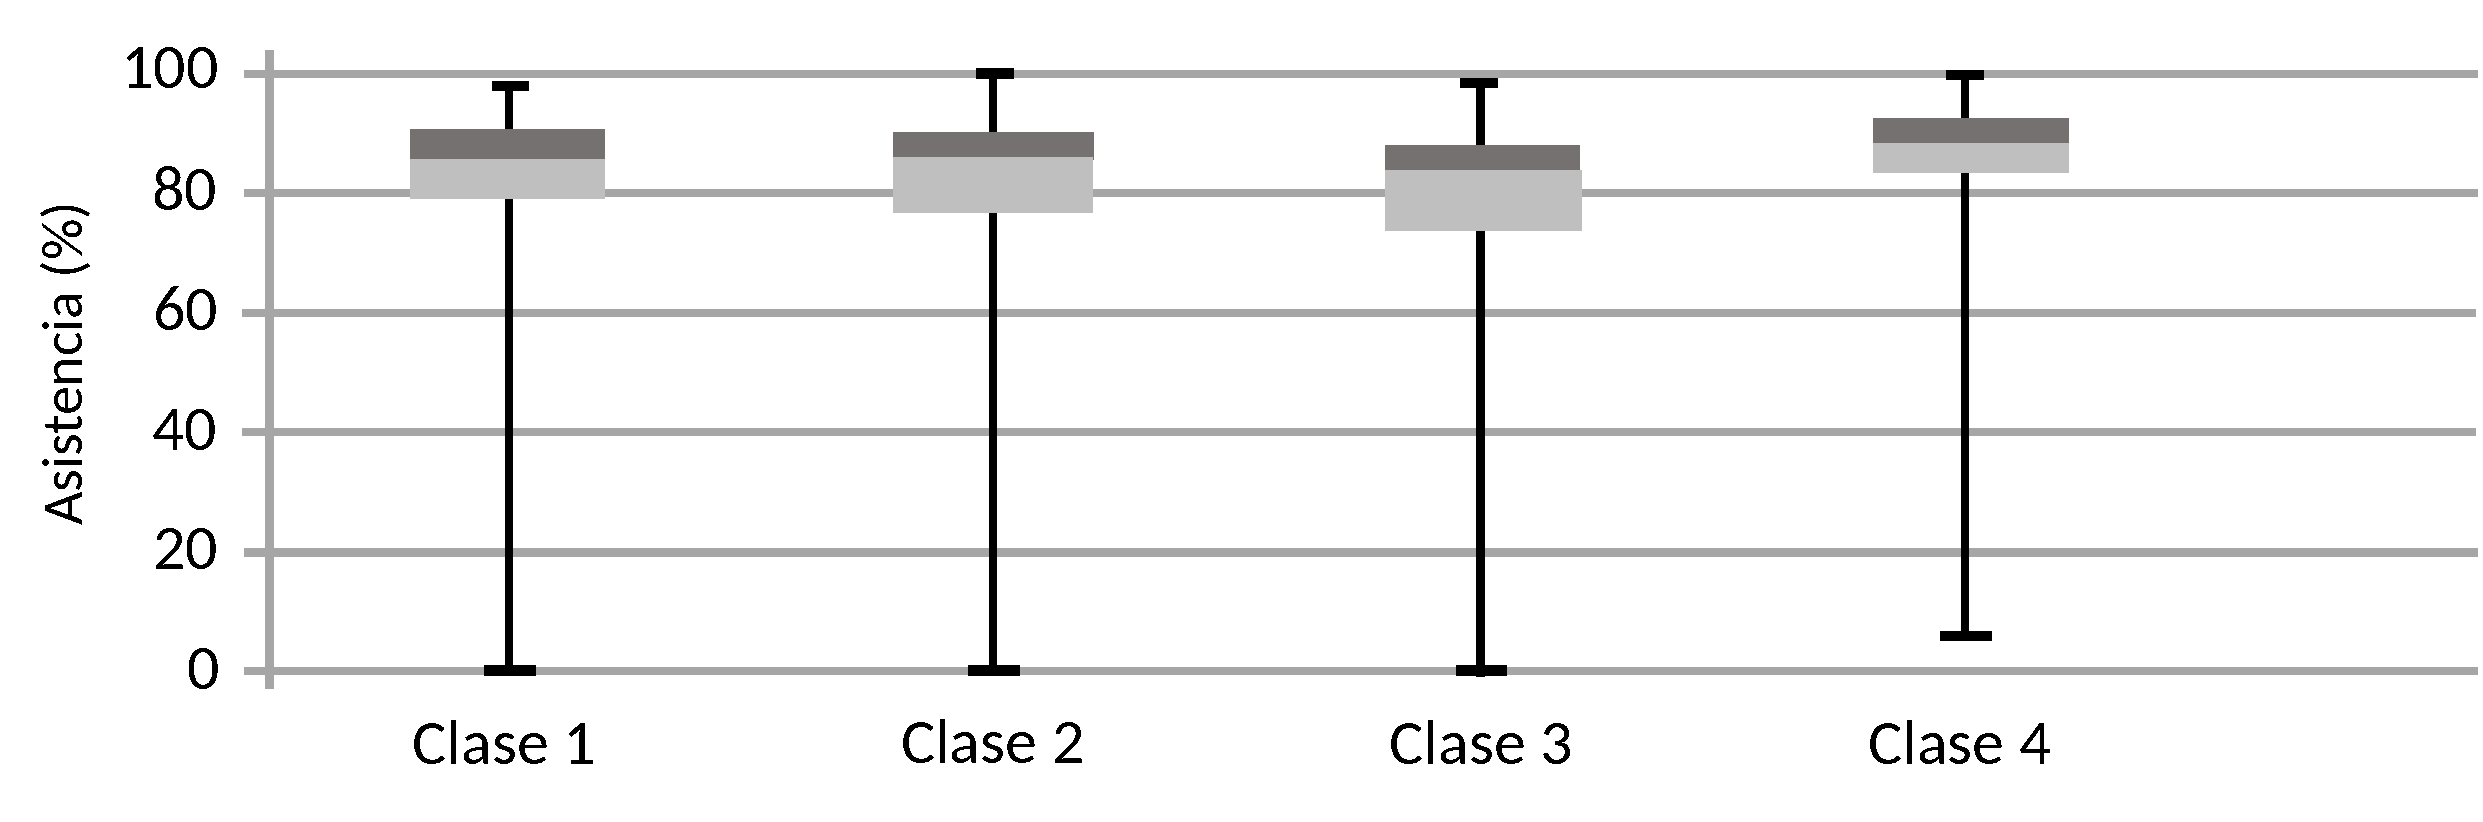
\includegraphics[width=0.75\textwidth]{images/fig-008.pdf}
 \caption{Caja y bigote de variable Asistencia, por cada grupo de estudiantes}
 \label{Figura 8}
 \source{Elaboración propia.}
\end{figure}

De acuerdo con lo anterior, se agruparon los alumnos según el comportamiento de las variables definidas como de mayor preponderancia: aquellos que no abandonan ya que poseen porcentajes adecuados de asistencia y asignaturas aprobadas, y los que presentan un nivel insuficiente en uno o los dos factores mencionados, llevándolos a abandonar.

Así, al utilizar los resultados obtenidos con el CJA, se establecen los perfiles descritos en la \Cref{Tabla 7}.

\begin{table}[htbp]
    \caption{Perfiles de estudiantes.}
    \label{Tabla 7}
    \centering
    \begin{tabular}{lp{9cm}}
    \toprule
    Perfil alumno & Descripción\\
    \midrule
    Bajo riesgo 4 & Alta probabilidad de ser retenidos de acuerdo con asistencia y aprobación de asignaturas. Además, al pertenecer a la clase 4, poseen un riesgo bajo.\\
    Bajo riesgo 1 & Alta probabilidad de ser retenidos de acuerdo con asistencia y aprobación de asignaturas. Además, al pertenecer a la clase 1, poseen un riesgo medio-bajo.\\
    Bajo riesgo 2 & Alta probabilidad de ser retenidos de acuerdo con asistencia y aprobación de asignaturas. Además, al pertenecer a la clase 2, poseen un riesgo medio-alto.\\
    Bajo riesgo 3 & Alta probabilidad de ser retenidos de acuerdo con asistencia y aprobación de asignaturas. Además, al pertenecer a la clase 3, poseen un riesgo alto.\\
    Alto riesgo 4 & Alta probabilidad de abandono de acuerdo con asistencia y aprobación de asignaturas. Además, al pertenecer a la clase 4, poseen un riesgo bajo.\\
    Alto riesgo 1 & Alta probabilidad de abandono de acuerdo con asistencia y aprobación de asignaturas. Además, al pertenecer a la clase 1, poseen un riesgo medio-bajo.\\
    Alto riesgo 2 & Alta probabilidad de abandono de acuerdo con asistencia y aprobación de asignaturas. Además, al pertenecer a la clase 2, poseen un riesgo medio-alto.\\
    Alto riesgo 3 & Alta probabilidad de abandono de acuerdo con asistencia y aprobación de asignaturas. Además, al pertenecer a la clase 3, poseen un riesgo alto.\\
    \bottomrule
    \end{tabular}
    \source{Elaboración propia}
\end{table}

Con las cuatro clases definidas, las trece variables de entrada y el programa 4eMka2, se obtienen las reglas de asociación por grupo mediante conjuntos aproximados, cuyos resultados se muestran en la \Cref{Tabla 8}.

\begin{table}[htbp]
    %\centering
    \caption{Resultado de la aplicación de la técnica de conjuntos aproximados a los cuatro grupos y 13 variables.}
    \label{Tabla 8}
    \centering
    \begin{tabular}{lllp{5cm}lll}
    \toprule
    Clase & Regla & Estado & Condiciones & Strength & Support & Coverage\\
    \midrule
    \multirow{6}{*}{1} &
    \multirow{2}{*}{1-1} &
    \multirow{2}{*}{Abandona}
     & Promedio Puntaje Leng. y Mat. <= 510 &
    \multirow{2}{*}{10,53~\%} &
    \multirow{2}{*}{14} &
    \multirow{2}{*}{133}\\
    & & & Asignaturas inscritas <= 7 & & &\\
    \cmidrule{2-7}
    & \multirow{2}{*}{1-2} &
    \multirow{2}{*}{Retenido}
     & Asignaturas inscritas >= 15 &
    \multirow{2}{*}{11,70~\%} &
    \multirow{2}{*}{31} &
    \multirow{2}{*}{265}\\
    & & & Asistencia >= 90~\% & & &\\
    \cmidrule{2-7}
    & \multirow{2}{*}{1-3} &
    \multirow{2}{*}{Retenido}
     & Puntaje de Cs. o Hist. >= 598 &
    \multirow{2}{*}{10,94~\%} &
    \multirow{2}{*}{29} &
    \multirow{2}{*}{265}\\
    & & & Asignaturas inscritas >= 9 & & &\\
    \cmidrule{1-7}
    % Clase 2:
    \multirow{9}{*}{2} &
    \multirow{3}{*}{2-1} &
    \multirow{3}{*}{Abandona}
     & Riesgo Ranking <= 1,0 &
    \multirow{3}{*}{16,24~\%} &
    \multirow{3}{*}{57} &
    \multirow{3}{*}{351}\\
    & & & Promedio Puntaje Leng. y Mat. <= 425 & & &\\
    & & & Asignaturas aprobadas <= 38~\% & & &\\
    \cmidrule{2-7}
    & \multirow{3}{*}{2-2} &
    \multirow{3}{*}{Abandona}
     & NEM <= 4,90 &
    \multirow{3}{*}{13,11~\%} &
    \multirow{3}{*}{46} &
    \multirow{3}{*}{351}\\
    & & & Asignaturas inscritas <= 7 & & &\\
    & & & Asistencia >= 81~\% & & &\\
    \cmidrule{2-7}
    & \multirow{3}{*}{2-3} &
    \multirow{3}{*}{Retenido}
     & NEM >= 5,30 &
    \multirow{3}{*}{9,82~\%} &
    \multirow{3}{*}{56} &
    \multirow{3}{*}{570}\\
    & & & Promedio Puntaje Leng. y Mat. >= 429 & & &\\
    & & & Asignaturas aprobadas >= 93~\% & & &\\
    \cmidrule{1-7}
    % Clase 3:
    \multirow{10}{*}{3} &
    \multirow{3}{*}{3-1} &
    \multirow{3}{*}{Abandona}
     & NEM <= 5,47 &
    \multirow{3}{*}{24,63~\%} &
    \multirow{3}{*}{101} &
    \multirow{3}{*}{410}\\
    & & & Puntaje de Cs. o Hist. <= 407 & & &\\
    & & & Asignaturas aprobadas <= 0~\% & & &\\
    \cmidrule{2-7}
    & \multirow{3}{*}{3-2} &
    \multirow{3}{*}{Abandona}
     & NEM <= 5,10 &
    \multirow{3}{*}{20,00~\%} &
    \multirow{3}{*}{82} &
    \multirow{3}{*}{410}\\
    & & & Asignaturas inscritas <= 8 & & &\\
    & & & Asistencia <= 71~\% & & &\\
    \cmidrule{2-7}
    & \multirow{4}{*}{3-3} &
    \multirow{4}{*}{Retenido}
     & Riesgo Ranking >= 2,0 &
    \multirow{4}{*}{14,47~\%} &
    \multirow{4}{*}{67} &
    \multirow{4}{*}{463}\\
    & & & Puntaje de Cs. o Hist. >= 384 & & &\\
    & & & Asignaturas inscritas >= 14 & & &\\
    & & & Asistencia >= 88~\% & & &\\
    \cmidrule{1-7}
    \multirow{6}{*}{4} &
    \multirow{2}{*}{4-1} &
    \multirow{2}{*}{Abandona}
     & Asignaturas inscritas <= 7 &
    \multirow{2}{*}{40,63~\%} &
    \multirow{2}{*}{26} &
    \multirow{2}{*}{64}\\
    & & & Asistencia <= 75~\% & & &\\
    \cmidrule{2-7}
    & \multirow{2}{*}{4-2} &
    \multirow{2}{*}{Abandona}
     & Asignaturas inscritas <= 7 &
    \multirow{2}{*}{35,94~\%} &
    \multirow{2}{*}{23} &
    \multirow{2}{*}{64}\\
    & & & Asignaturas aprobadas <= 0~\% & & &\\
    \cmidrule{2-7}
    & \multirow{2}{*}{4-3} &
    \multirow{2}{*}{Retenido}
     & Riesgo Ranking >= 598 &
    \multirow{2}{*}{35,14~\%} &
    \multirow{2}{*}{65} &
    \multirow{2}{*}{185}\\
    & & & Asignaturas inscritas >= 15 & & &\\
    
    \bottomrule
    \end{tabular}
    \source{Elaboración propia}
\end{table}

Debido a la baja solidez (strength) de las 12 reglas obtenidas, y del mismo modo que en la etapa del clustering, se decidió profundizar el análisis obteniendo de manera independiente las reglas de decisión para estudiantes que abandonan y los que no (\Cref{Tabla 9}).

\begin{table}[htbp]
    \caption{Resultado de la aplicación de la técnica de conjuntos aproximados a los cuatro grupos y 13 variables, por condición de deserción.}
    \label{Tabla 9}
    \centering
    \begin{tabular}{lllp{5cm}lll}
    \toprule
    Clase & Subclase & Regla & Condiciones & Strength & Support & Coverage\\
    \midrule
    \multirow{4}{*}{1} & Abandonan & 1-1 & Puntaje de Cs. o Hist. <= 585 & 83,86~\% & 256 & 305\\
    \cmidrule{2-7}
    & \multirow{3}{*}{Retenidos} & 1-2 & Asistencia >= 36~\% & 100,00~\% & 715 & 715\\
    & & 1-3 & Asignaturas aprobadas >= 40~\% & 96,78~\% & 692 & 715\\
    & & 1-4 & Asignaturas inscritas >= 7 & 94,97~\% & 679 & 715\\
    \cmidrule{1-7}
    % Grupo 2:
    \multirow{5}{*}{2} &
    \multirow{2}{*}{Abandonan} & 2-1 & Promedio Puntaje Leng. y Mat. <= 498 & 81,07~\% & 882 & 1088\\
    & & 2-2 & Asignaturas inscritas <= 10 & 66,08~\% & 719 & 1088\\
    \cmidrule{2-7}
    & \multirow{3}{*}{Retenidos} & 2-3 & Asistencia >= 41~\% & 99,69~\% & 1949 & 1955\\
    & & 2-4 & Asignaturas aprobadas >=27~\% & 97,80~\% & 1912 & 1955\\
    & & 2-5 & Asignaturas inscritas >=7~\% & 96,06~\% & 1878 & 1955\\
    \cmidrule{1-7}
   % Grupo 3:
    \multirow{5}{*}{3} &
    \multirow{2}{*}{Abandonan} & 3-1 & Puntaje de Cs. o Hist. <= 477 & 97,94~\% & 667 & 681\\
    & & 3-2 & Asignaturas inscritas <= 10 & 66,67~\% & 453 & 679\\
    \cmidrule{2-7}
    & \multirow{3}{*}{Retenidos} & 3-3 & Asistencia >= 49~\% & 99,66~\% & 875 & 878\\
    & & 3-4 & Asignaturas inscritas >=7~\% & 96,01~\% & 843 & 878\\
    & & 3-5 & Asignaturas aprobadas >=36~\% & 95,90~\% & 842 & 878\\
    \cmidrule{1-7}
    % Grupo 4:
    \multirow{5}{*}{4} &
    \multirow{3}{*}{Abandonan} & 4-1 & Promedio Puntaje Leng. y Mat. <= 720 & 96,60~\% & 142 & 147\\
    & & 4-2 & Puntaje de Cs. o Hist. <= 714 & 93,20~\% & 137 & 147\\
    & & 4-3 & Asignaturas aprobadas <= 93~\% & 65,31~\% & 96 & 147\\
    \cmidrule{2-7}
    & \multirow{2}{*}{Retenidos} & 4-4 & Asignaturas inscritas >= 8 & 97,05~\% & 427 & 440\\
    & & 4-5 & Asistencia >=77~\% & 96,36~\% & 424 & 440\\
    \bottomrule
    \end{tabular}
    \source{Elaboración propia}
\end{table}

Del análisis conjunto de las reglas de asociación con mayor consistencia (strength > 80~\%), obtenidas para los alumnos de primer año que abandonan, se obtiene que las variables que presentan una mayor incidencia en esta decisión están ligadas a factores previos al ingreso (Promedio Puntaje Lenguaje y Matemática, Puntaje de Ciencias o Historia). Este mismo análisis en los estudiantes que son retenidos muestra que las variables más influyentes están relacionadas con factores de posingreso a estudios superiores (Asistencia, Asignaturas aprobadas, Asignaturas inscritas).

Así, al no encontrar variables cuyas reglas permitan explicar de forma transversal el hecho que un estudiante decida abandonar o no, independientemente de la clase a la que pertenece, se realizó un último análisis. Se buscan reglas de asociación tomando como variable decisional la clase a la que pertenece el estudiante (\Cref{Tabla 10}) y no la variable Abandono. De esta forma se puede verificar la complementariedad existente entre los distintos grupos.

\begin{table}[htbp]
    \caption{Resultado de la aplicación de la técnica de conjuntos aproximados a los cuatro grupos y 13 variables, por grupo.}
    \label{Tabla 10}
    \centering
    \begin{tabular}{llp{5cm}lll}
    \toprule
    Clase & Regla & Condiciones & Strength & Support & Coverage\\
    \midrule
    1 & 1-1 & Asignaturas inscritas <= 10 & 77,48~\% & 320 & 413\\
    \cmidrule{1-6}
    \multirow{2}{*}{2} & 2-1 & Asistencia >= 51~\% & 93,52 & 2885 & 3085\\
    & 2-2 & Asignaturas aprobadas >= 42~\% & 79,48~\% & 2452 & 3085\\
    \cmidrule{1-6}
    \multirow{3}{*}{3} & 3-1 & Asignaturas inscritas >= 6 & 93,65 & 1446 & 1544\\
    & 3-2 & Asistencia >= 38~\% & 96,05~\% & 1483 & 1544\\
    & 3-3 & Asignaturas aprobadas >= 43~\% & 71,05~\% & 1097 & 1544\\
    \cmidrule{1-6}
    \multirow{5}{*}{4} & 4-1 & Promedio Puntaje Leng. y Mat. <= 572 & 97,61 & 573 & 587\\
    & 4-2 & Asignaturas inscritas >= 6 & 96,93~\% & 569 & 587\\
    & 4-3 & Puntaje de Cs. o Hist. >= 588 & 79,22~\% & 465 & 587\\
    & 4-4 & Asignaturas aprobadas >= 45~\% & 93,02~\% & 546 & 587\\
    & 4-5 & Asistencia >= 50~\% & 91,82~\% & 539 & 587\\
    \bottomrule
    \end{tabular}
    \source{Elaboración propia}
\end{table}

Se observa que existe cierta complementariedad entre los factores que definen cada grupo, los cuales se repiten entre clases. La complementariedad se define por los factores relacionados al desarrollo del estudiante posingreso a su primer año de ES. Sin embargo, los valores obtenidos en estas reglas no permiten definir una clara demarcación entre los valores que definen a cada clase, para validar con la información disponible no es posible desarrollar un modelo que pueda explicar la deserción.

Con esto, se valida la importancia que Asistencia y Asignaturas aprobadas tienen en el proceso de gestión estudiantil, y por consecuencia, en el manejo del abandono, sin embargo, no poseen la incidencia suficiente como para explicar el fenómeno por sí solas.

Finalmente, al considerar los perfiles de estudiantes 1, 2, 3 y 4 (\Cref{Tabla 5}), que tienen una dificultad de retención baja, alta, muy alta, y muy baja, respectivamente, y las reglas de asociación obtenidas para cada grupo (\Cref{Tabla 9,Tabla 10}), se propone un modelo de gestión estudiantil basado en el trabajo colaborativo de distintas unidades académicas en dos ámbitos: mitigación del abandono (\cref{Figura 9}) y fomento de la retención (\cref{Figura 10}). Para mitigar el abandono, se proponen cursos de nivelación obligatorios para los estudiantes con déficit en los resultados de sus pruebas de selección (\Cref{Tabla 9}), donde se desarrollen competencias académicas, valores y habilidades sociales.

\begin{figure}[htbp]
 \centering
 \caption{Modelo de gestión estudiantil para disminuir el abandono}
 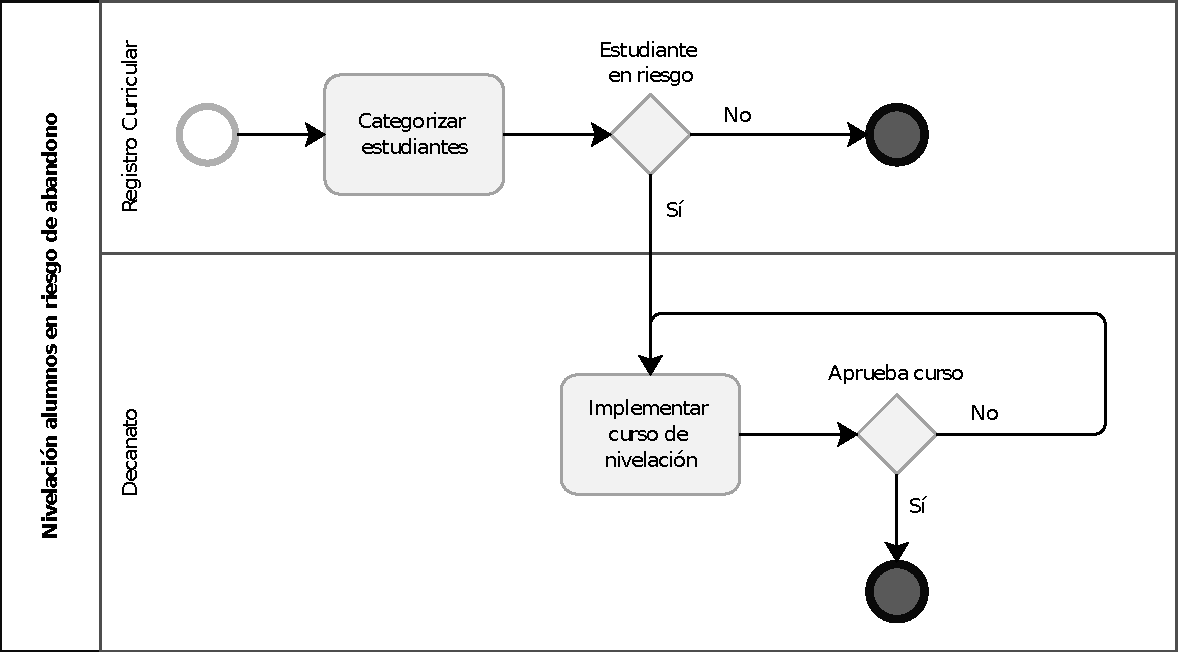
\includegraphics[width=0.65\textwidth]{images/fig-009.pdf}
 \label{Figura 9}
 \source{Elaboración propia.}
\end{figure}

\begin{figure}[htbp]
 \centering
 \caption{Modelo de gestión estudiantil para fomentar la retención}
 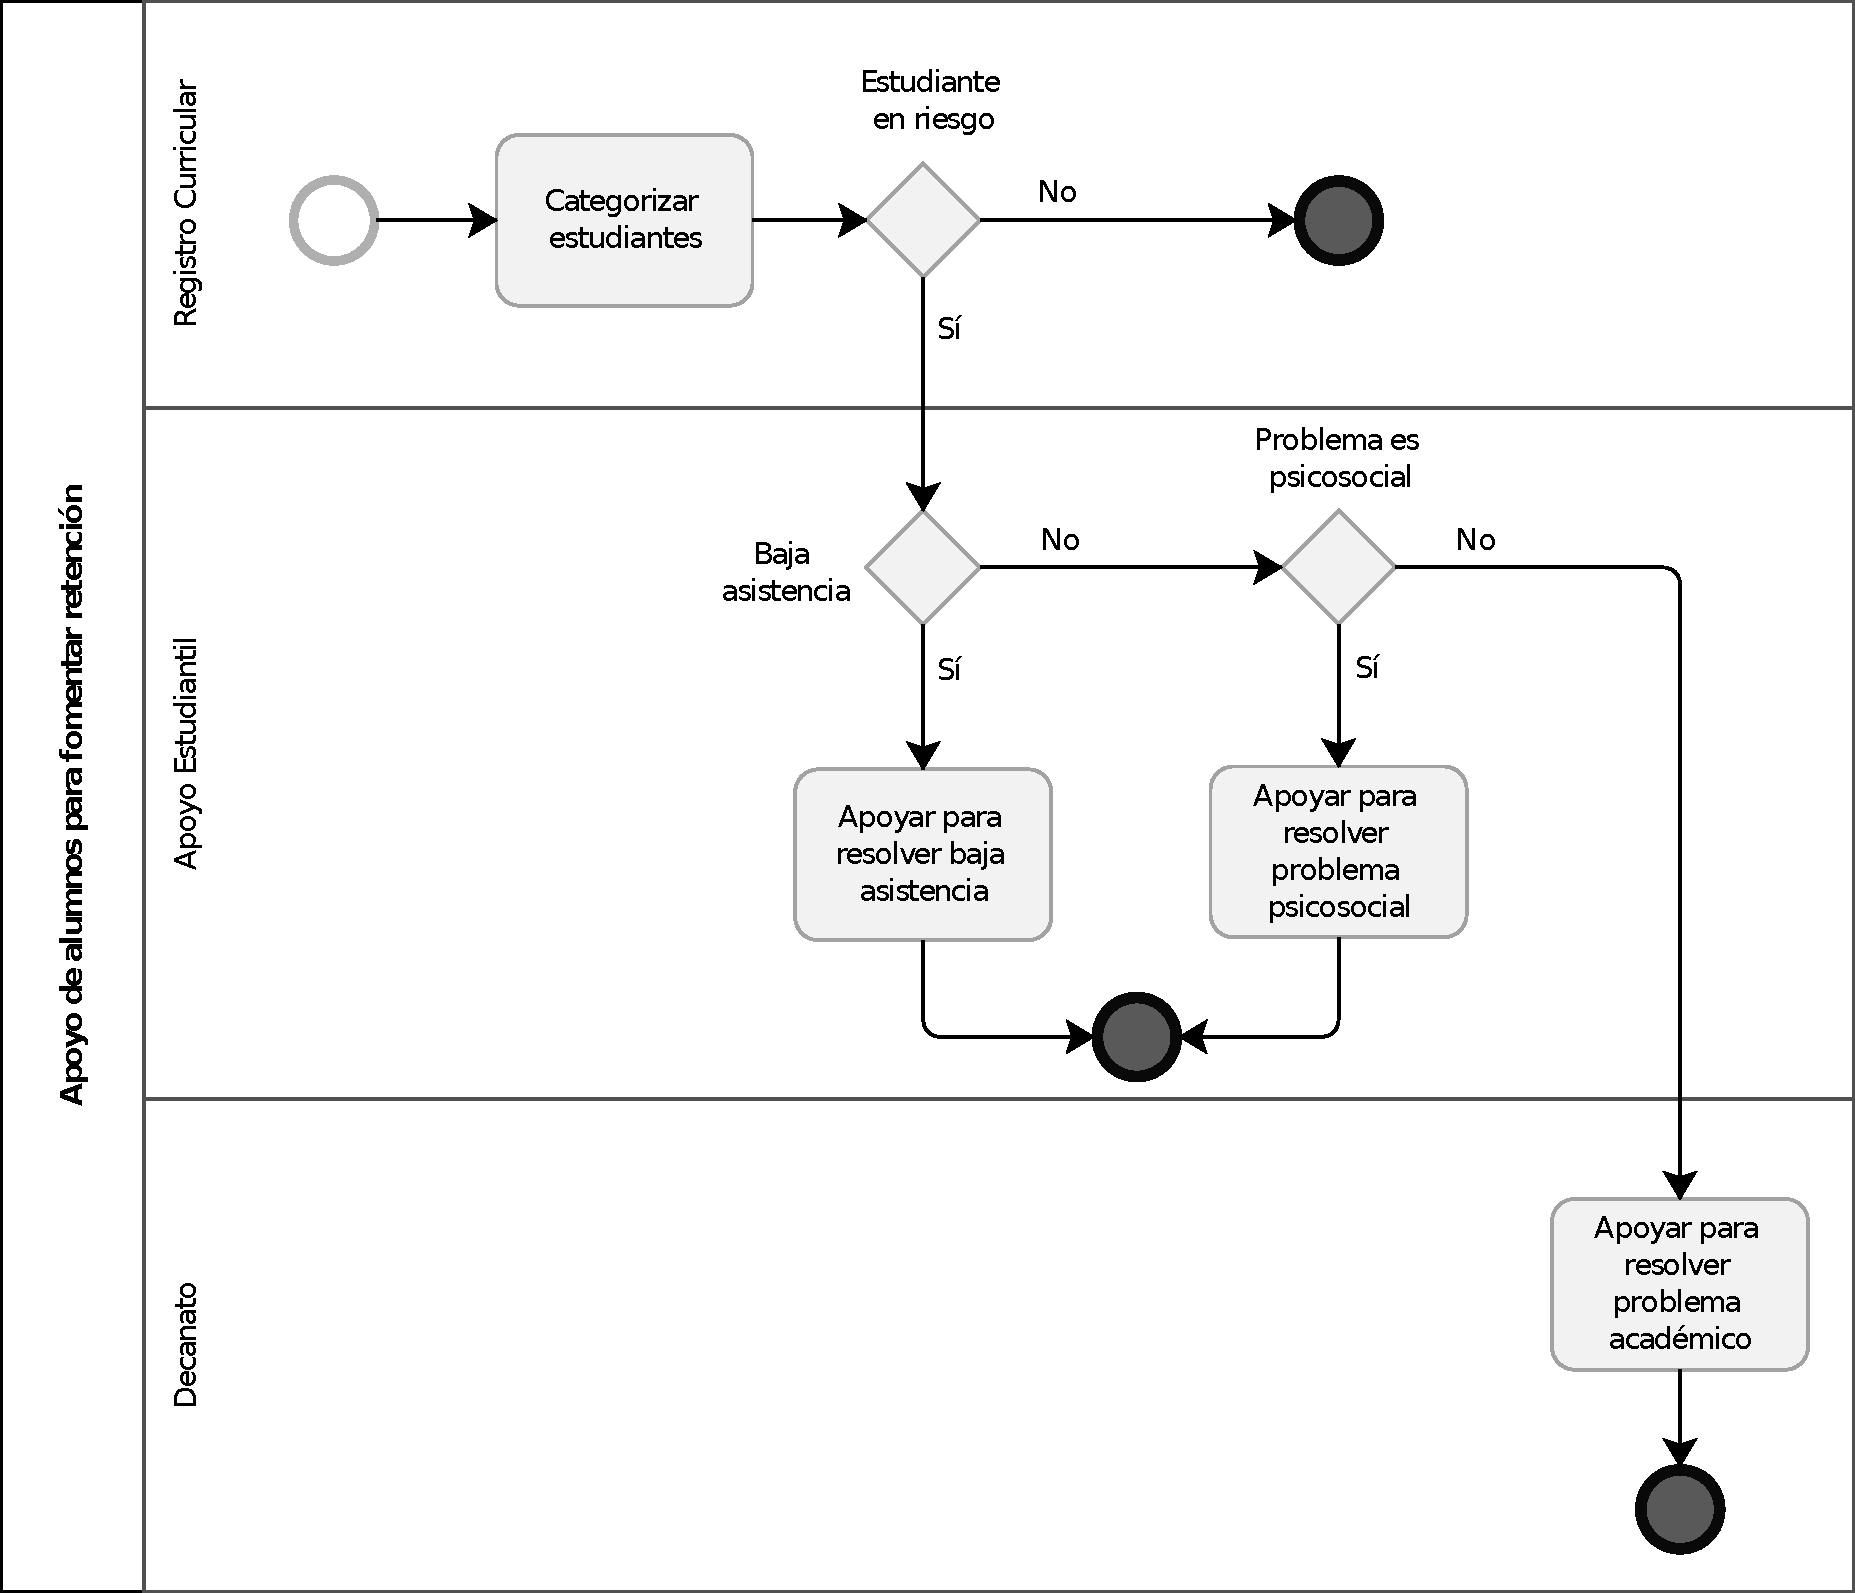
\includegraphics[width=0.65\textwidth]{images/fig-010}
 \label{Figura 10}
 \source{Elaboración propia}
\end{figure}

Para fomentar la retención, según factores ligados al posingreso (\Cref{Tabla 9}), Registro Curricular monitoreará la asistencia, inscripción y aprobación de asignaturas, y derivará a los alumnos a distintas unidades académicas, según sea el problema. A los estudiantes con baja asistencia los conducirá a una unidad de Apoyo Estudiantil, que indagará las causas y brindará el apoyo, ya sea psicológico o financiero. A quienes presenten baja inscripción de asignaturas se derivan a Apoyo Estudiantil o al Decanato (Dirección de Carrera), según su necesidad es psicosocial o académica, respectivamente. Y a los estudiantes, según porcentaje de aprobación, los derivará a Apoyo Estudiantil o al Decanato.


\section{Conclusiones}\label{sec-organizacao}

La presente investigación valida una metodología basada en CRISP-DM, correlación y aprendizaje no supervisado, para obtener perfiles de estudiantes en riesgo de abandono. Así, permite proponer mejoras en la gestión estudiantil, que propenden a disminuir este riesgo.

Por otro lado, no se pudo generar un modelo explicativo de la deserción dado que, al utilizar registros históricos, la información se restringió solo a los datos disponibles. Esto representa una oportunidad de mejora, y demuestra la importancia de implementar sistemas de información institucionales que contengan los datos socioeconómicos, demográficos, psicosociales y académicos necesarios de los estudiantes.

La variedad de enfoques y heterogeneidad de los factores involucrados en el fenómeno del abandono estudiantil hacen de su análisis un trabajo muy dependiente del contexto en el cual se lleva a cabo. El estudio se realizó con estudiantes de primer año de pregrado en jornada diurna de una universidad privada independiente chilena y no adscrita al Sistema de acceso universitario. Así, la comparación de los resultados obtenidos con los de otros estudios es pertinente y válida en tanto se trate del mismo tipo de institución, área de conocimientos, tipo de estudiante, entorno social, entre otros. En base a lo anterior, se puede afirmar que en el contexto estudiado las variables que presentan una mayor incidencia en la decisión de abandonar están ligadas a factores previos al ingreso (puntajes en pruebas de selección y NEM) y académicas posingreso (Asignaturas aprobadas y Asistencia). Esto se correlaciona con lo encontrado por \cite{BarriosF2011,Larroucau2015,Carvajal2018,Velasquez2014}, y especialmente con \cite{Miranda2017}, que es la investigación más afín.

El presente estudio innova en su contexto en la incorporación de la variable Aprobación de asignaturas, y en el uso del clustering jerárquico aglomerativo y de los conjuntos aproximados para encontrar perfiles de estudiantes en riesgo de abandono y los respectivos factores predominantes.

Por último, los resultados de esta investigación contribuyen al desarrollo de la teoría del abandono estudiantil en las universidades chilenas, a su gestión, y establece un fundamento metodológico para futuros estudios empíricos.

\printbibliography


%\begin{lstlisting}[language=tex, label=lst-contributions, caption={Contribuição dos autores.}]
\begin{contributors}[sec-contributors]
\authorcontribution{Mauricio Hinojosa V.}[funding, software, validation, writing, review]
\authorcontribution{Iván Derpich}[conceptualization, supervision]
\authorcontribution{Miguel Alfaro}[projadm, supervision]
\authorcontribution{David Ruete}[datacuration, formalanalysis, funding, methodology, resources, validation]
\authorcontribution{Alejandro Caroca}[conceptualization, resources, validation]
\authorcontribution{Gustavo Gatica}[datacuration, formalanalysis, methodology, projadm, software, supervision, review]
\end{contributors}
%\end{lstlisting} %stopzone


%\appendix 
\end{document}

